% !TeX encoding = UTF-8
% !TeX spellcheck = en_US

\documentclass[11pt,oneside,a4paper]{memoir}

% General
\usepackage[utf8]{inputenc}
\usepackage[shorthands=off,english]{babel}
\usepackage{hyperref}
\usepackage{titlesec} 
\usepackage{tabulary}
\usepackage{enumitem}
\setlist{nosep, leftmargin=4em}

% Maths
\usepackage{amsmath}
\usepackage{amsfonts} % caligraphic fonts
\usepackage{amssymb}  % symbols
\usepackage{empheq}   % frame equations
\usepackage{siunitx}  % correct units

% Pictures
\usepackage{graphicx}
\usepackage{caption}
\usepackage{subcaption}
\usepackage{rotating}
\usepackage{epstopdf}
\usepackage{tikz}
\usetikzlibrary{shapes,arrows,positioning}

% Should be loaded last
\usepackage{setspace}
\usepackage[noabbrev]{cleveref}

% Default fixed font does  support bold face

% Custom colors
\usepackage{color}
\definecolor{deepblue}{rgb}{0,0,0.5}
\definecolor{deepred}{rgb}{0.6,0,0}
\definecolor{deepgreen}{rgb}{0,0.5,0}
\definecolor{gray}{rgb}{0.5,0.5,0.4}

\usepackage{listings}
\usepackage{lstautogobble}
\renewcommand{\lstlistingname}{Code example}

% Python style for highlighting
\newcommand\pythonstyle{\lstset{
    language=Python,
    basicstyle=\linespread{1}\footnotesize\ttfamily,
    otherkeywords={self},             % Add keywords here
    keywordstyle=\footnotesize\ttfamily\bfseries\color{deepblue},
    emph={MyClass,__init__},          % Custom highlighting
    emphstyle=\bf\color{deepred},    % Custom highlighting style
    stringstyle=\color{deepgreen},
    frame=tb,                         % Any extra options here
    showstringspaces=false,           % 
    tabsize=4,
    numbers=left,    
    numberstyle=\tiny\color{gray}, 
    breaklines=true,
    autogobble=true,
    commentstyle=\color{gray},           
}}


% Python environment
\lstnewenvironment{python}[1][]
{
\pythonstyle
\lstset{#1}
}
{}

% Python for external files
\newcommand\pythonexternal[2][]{{
\pythonstyle
\lstinputlisting[#1]{#2}}}

\newcommand\cppstyle{\lstset{
    language=C++,
    basicstyle=\ttfamily,
    keywordstyle=\color{deepblue}\ttfamily,
    stringstyle=\color{red}\ttfamily,
    commentstyle=\color{grey}\ttfamily,
    morecomment=[l][\color{magenta}]{\#},
    autogobble=true,
}}

% C++ environment
\lstnewenvironment{c++}[1][]
{
    \cppstyle
    \lstset{#1}
}
{}

% % % % % % % % % % % % % % % % % %
% trick not to release comments   %
  \newif\ifdraft
%	                              %
	%\releasefalse
	\drafttrue
%	                              %
	\ifdraft
		\usepackage[colorinlistoftodos,textsize=scriptsize]{todonotes}
	\fi
% end of trick                    %
% % % % % % % % % % % % % % % % % %

\renewcommand{\vec}[1]{\underline{#1}}
\newcommand{\mat}[1]{\underline{\underline{#1}}}
\newcommand{\scal}[2]{\langle #1 {\,,\,} #2 \rangle}
\newcommand{\Real}[1]{\mathcal{R}e\left(#1\right)}
\newcommand{\Imag}[1]{\mathcal{I}m\left(#1\right)}
\newcommand{\remark}{\paragraph{Remark ---}}
\setsecnumdepth{subsubsection}
%\maxtocdepth{subsection}
\renewcommand{\baselinestretch}{1.5} 
\setlrmarginsandblock{3cm}{2.5cm}{*}
\setulmarginsandblock{3cm}{2.5cm}{*}
\checkandfixthelayout

\def\thetitle{Localization and correction of orbit perturbations in BESSY II storage ring}
\def\thesubject{Master Thesis}
\def\theauthor{Olivier Churlaud}
\def\theauthorinfo{Matriculation number: 366\,964}
\author{\theauthor}
\title{\thetitle}

\hypersetup{
    unicode=true,
    pdftitle={\thetitle},
    pdfauthor={\theauthor},
    pdfsubject={\thesubject},
    colorlinks=true,       % false: boxed links; true: colored links
    linkcolor=teal,       % color of internal links (change box color with linkbordercolor)
    citecolor=olive,
    filecolor=red,
    urlcolor=blue
}

\begin{document}

\frontmatter
\cleardoublepage
\thispagestyle{empty}

% !TeX encoding = UTF-8
% !TeX spellcheck = en_US
% !TeX root = ../main.tex

\begin{titlingpage}
	\noindent
	\begin{minipage}[t]{\textwidth}
		\flushright
		\begin{minipage}[c]{0.6\linewidth}
			\flushright
			\begin{SingleSpace}
				Technische Universität Berlin \\
				Fakultät IV - Elektrotechnik und Informatik  \\
				Institut für Energie- und Automatisierungstechnik \\
				Fachgebiet Regelungssysteme  \\
				Prof. Dr.-Ing. Jörg Raisch
			\end{SingleSpace}
		\end{minipage}
		\hspace{2em}
		\begin{minipage}[c]{3.2cm}
			
\includegraphics[width=1\linewidth]{img/tu-logo}
		\end{minipage}
	\end{minipage}
	
	\vfill

	\begin{center}
	\LARGE \textsc{\thesubject}
	\end{center}
	
	~
	
	\begin{Spacing}{3}
		\centering\textsc{\huge\thetitle}
	\end{Spacing}
	
	\vfill
	
	\centering	
	Submitted by
	

	\theauthor  ~-- \theauthorinfo

	~
	
	In partial fulfillment of the requirements for \\ the Degree of Master of Science in Electrical Engineering

	~
	
	
	\today		
	
	\vfill		


	Supervisors
	
	~
	
	\setlength{\tabcolsep}{15pt}
	\begin{tabular}{l l}
		TU Berlin
		&Prof. Dr.-Ing. Jörg Raisch \\
	    ~ & ~\\
			Helmholtz-Zentrum Berlin 
		& Prof. Dr. Andreas Jankowiak \\
		~ & Dr. Andreas Schälicke
	\end{tabular}
\end{titlingpage}

\ifdraft
	\listoftodos
\fi

\cleardoublepage
\begin{abstract}
       ......
\end{abstract}
\vfill

\cleardoublepage
\tableofcontents*
\listoffigures*

\mainmatter

% !TeX encoding = UTF-8
% !TeX spellcheck = en_US
% !TeX root = ../MasterThesis_OlivierChurlaud_2016.tex

\chapter{Introduction}
\label{sec:background}

\section{BESSY II -- General presentation}
BESSY II (\textbf{B}erliner \textbf{E}lektronen \textbf{S}peicherring-Gesellschaft für \textbf{Sy}n\-chro\-tron\-strahlung m.b.H.) is Berlin's electron storage ring, aimed at producing high energy light rays by synchrotron radiation. It emits extremely brilliant photons pulses ranging from Terahertz to hard X rays, with an emphasis on the soft X-ray range ~\cite{web:bessy_homepage}.

Scientific projects can freely apply for beam time at an experimental station, where they are able to adjust the wavelength, polarization and photon energy. More than 2000 scientists are using BESSY II equipment every year.

The storage ring has a circumference of \SI{240}{\meter} and provides around 50 beamlines (paths of light rays between the storage ring and experimentation stations). The electrons are accelerated to an energy up to \SI{1.7}{\giga\electronvolt}.

BESSY II was inaugurated in 1998 to let scientists study material structures and processes. Since 2009 it is a facility of the \textit{Helmholtz-Zentrum Berlin für Materialien und Energie} (HZB)

In addition to the guest scientists, operators and researchers work to ensure the good functioning of the whole facility and work on refining the quality and the stability of the light rays.

\section{BESSY II -- General functioning}
In the BESSY II  accelerator, particles are circularly accelerated in the same direction. The goal is to produce light, instead of collisions.

BESSY II functions based on the synchrotron radiation phenomenon: any accelerated particle emits radiations (in the form of photons). It can be shown~\cite{book:wille} that the radiated power in circular acceleration can be given as
\begin{equation}
P_s = \frac{e^2 c}{6 \pi \varepsilon_0}\frac{1}{(m_0 c^2)^4}\frac{E^4}{R^2}.
\end{equation}
where $c$ is the speed of light, $m_0$ the rest mass (independent of the velocity) of the particle, $e$ its charge, $E$ its energy, $R$ the bending radius and $\varepsilon_0$ the  vacuum permittivity.

Considering their low mass, electrons are very good candidates to produce high energy radiation (in comparison, accelerated protons would provide $10^{13}$ less radiation than electrons), and are therefore used in BESSY~II.

\begin{figure}
    \centering
    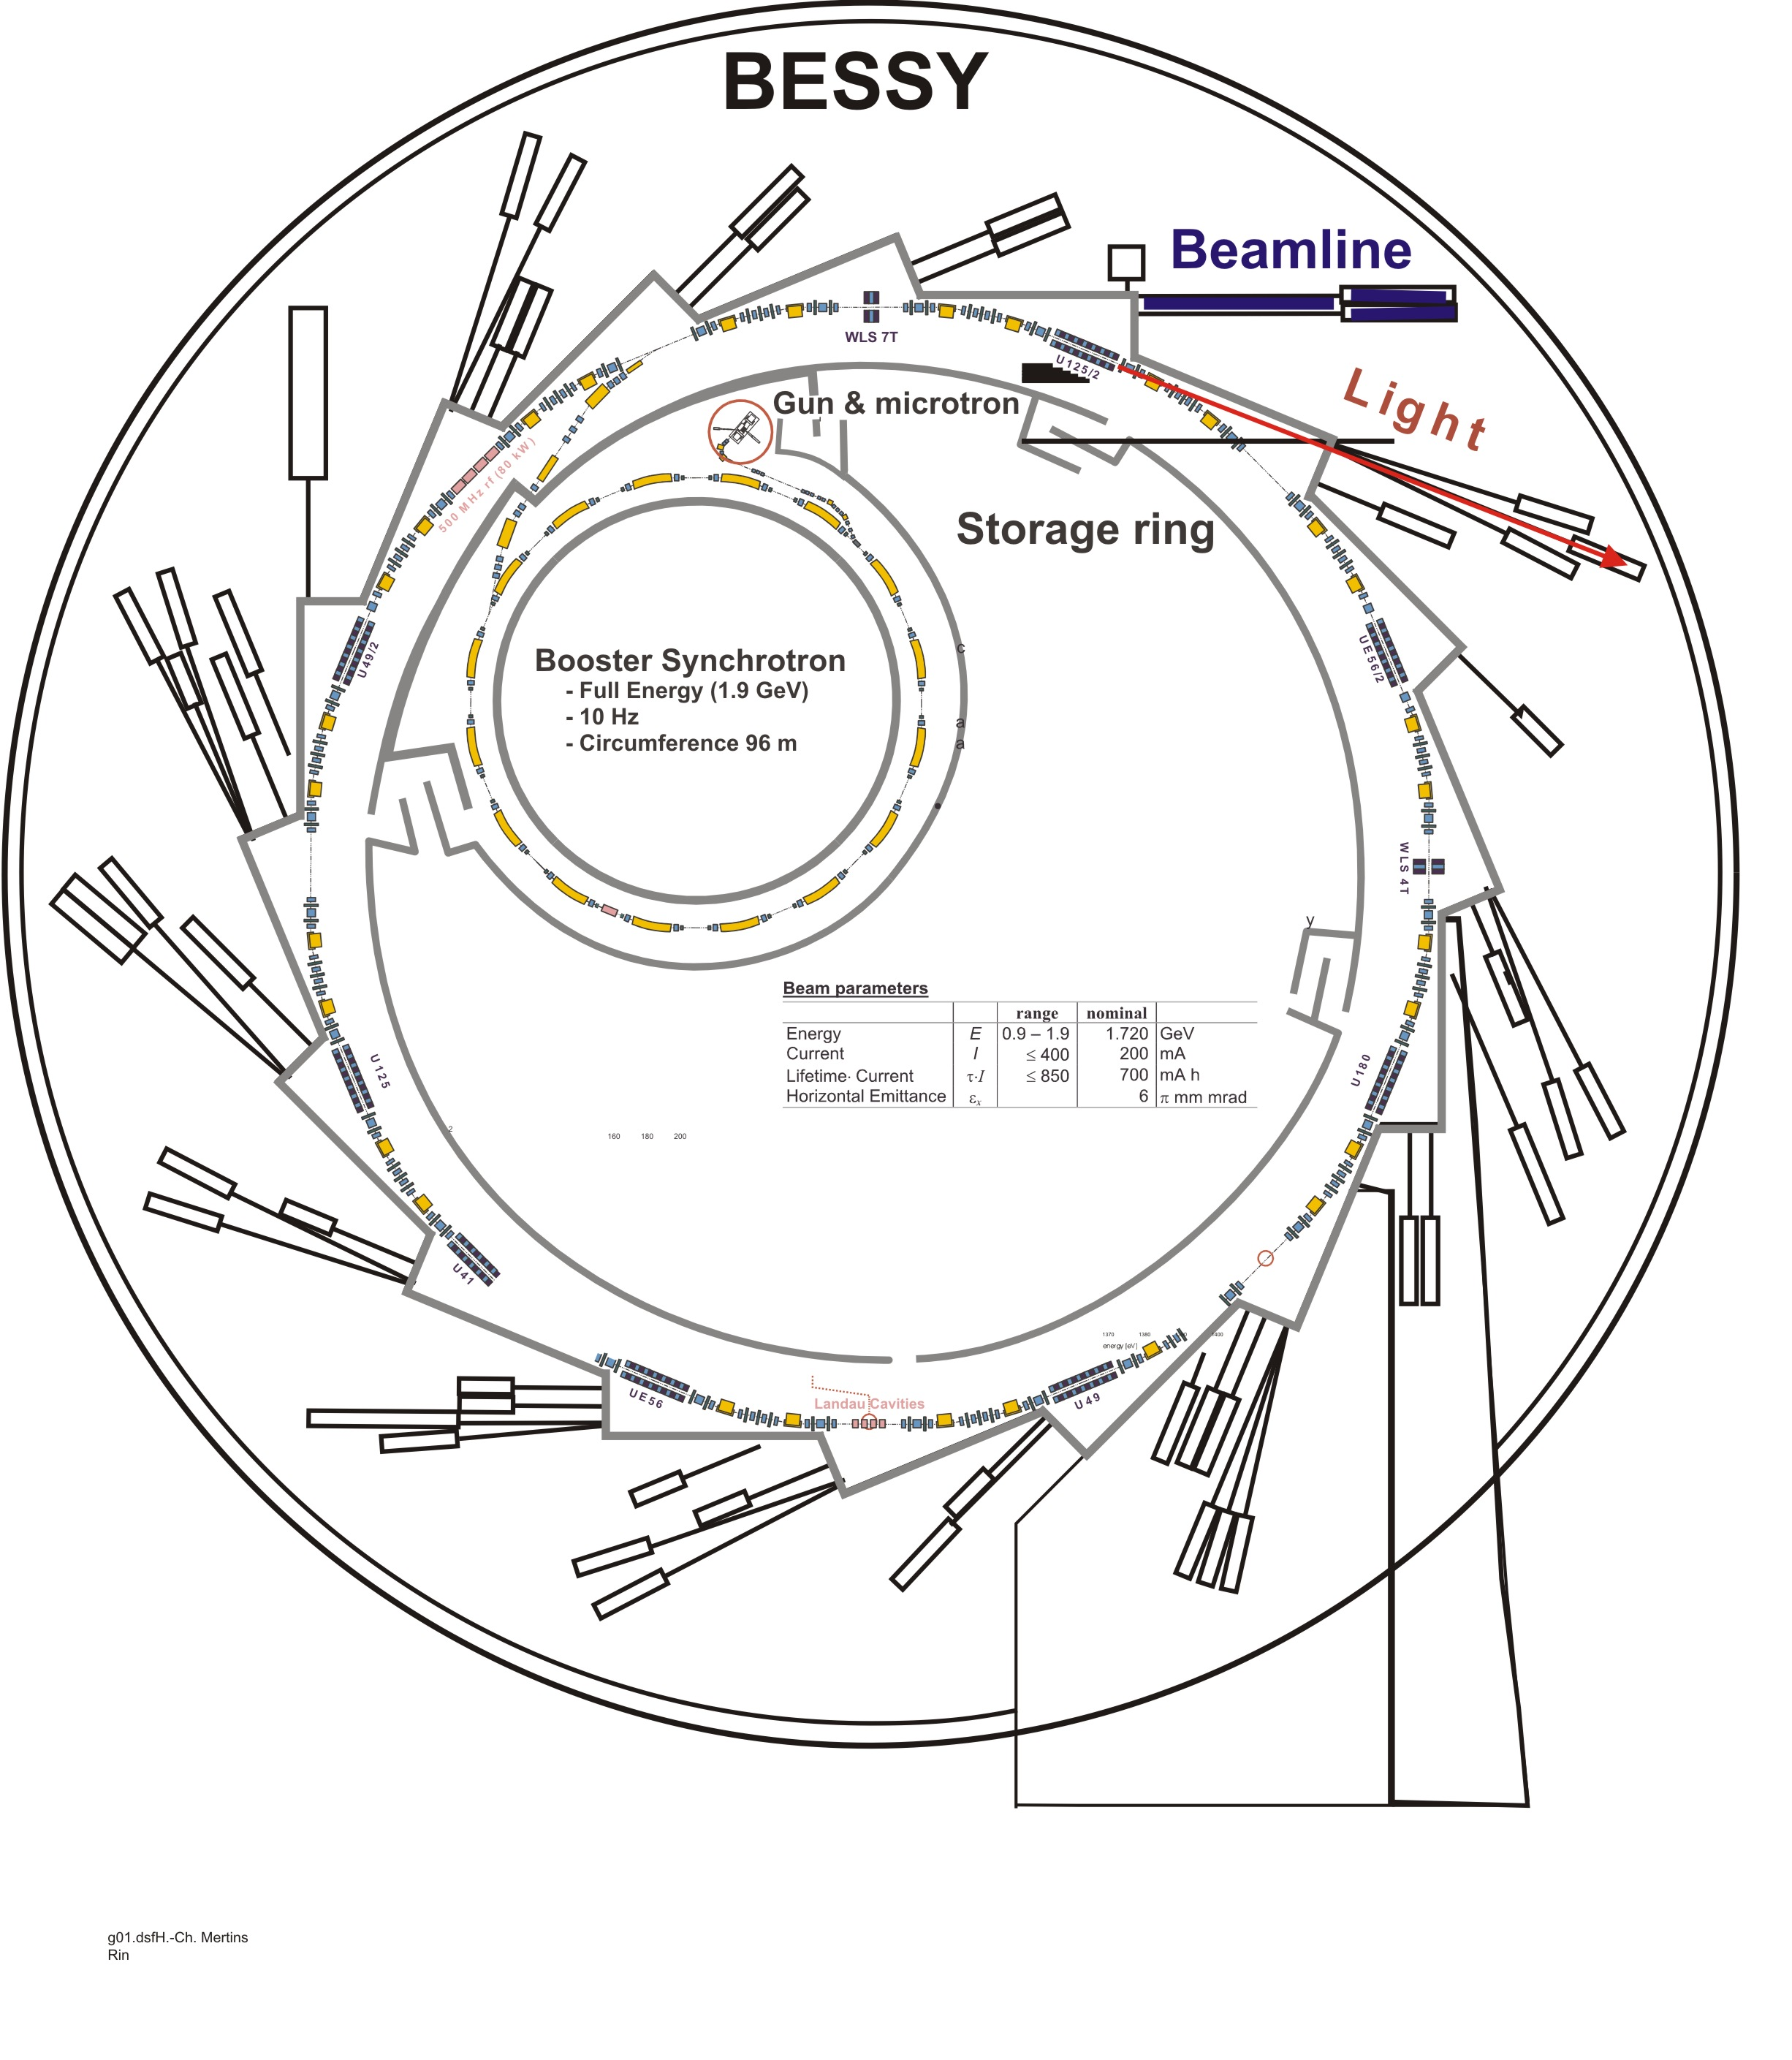
\includegraphics[width=0.8\textwidth]{img/bessy_acc_chain_web.jpg}
    \caption[BESSY~II -- Accelerator chain]{\label{fig:bessy_acc_web_simple} BESSY~II -- Accelerator chain (Source:~\cite{web:bessy_homepage})}
\end{figure}

\begin{sidewaysfigure}
    \centering
    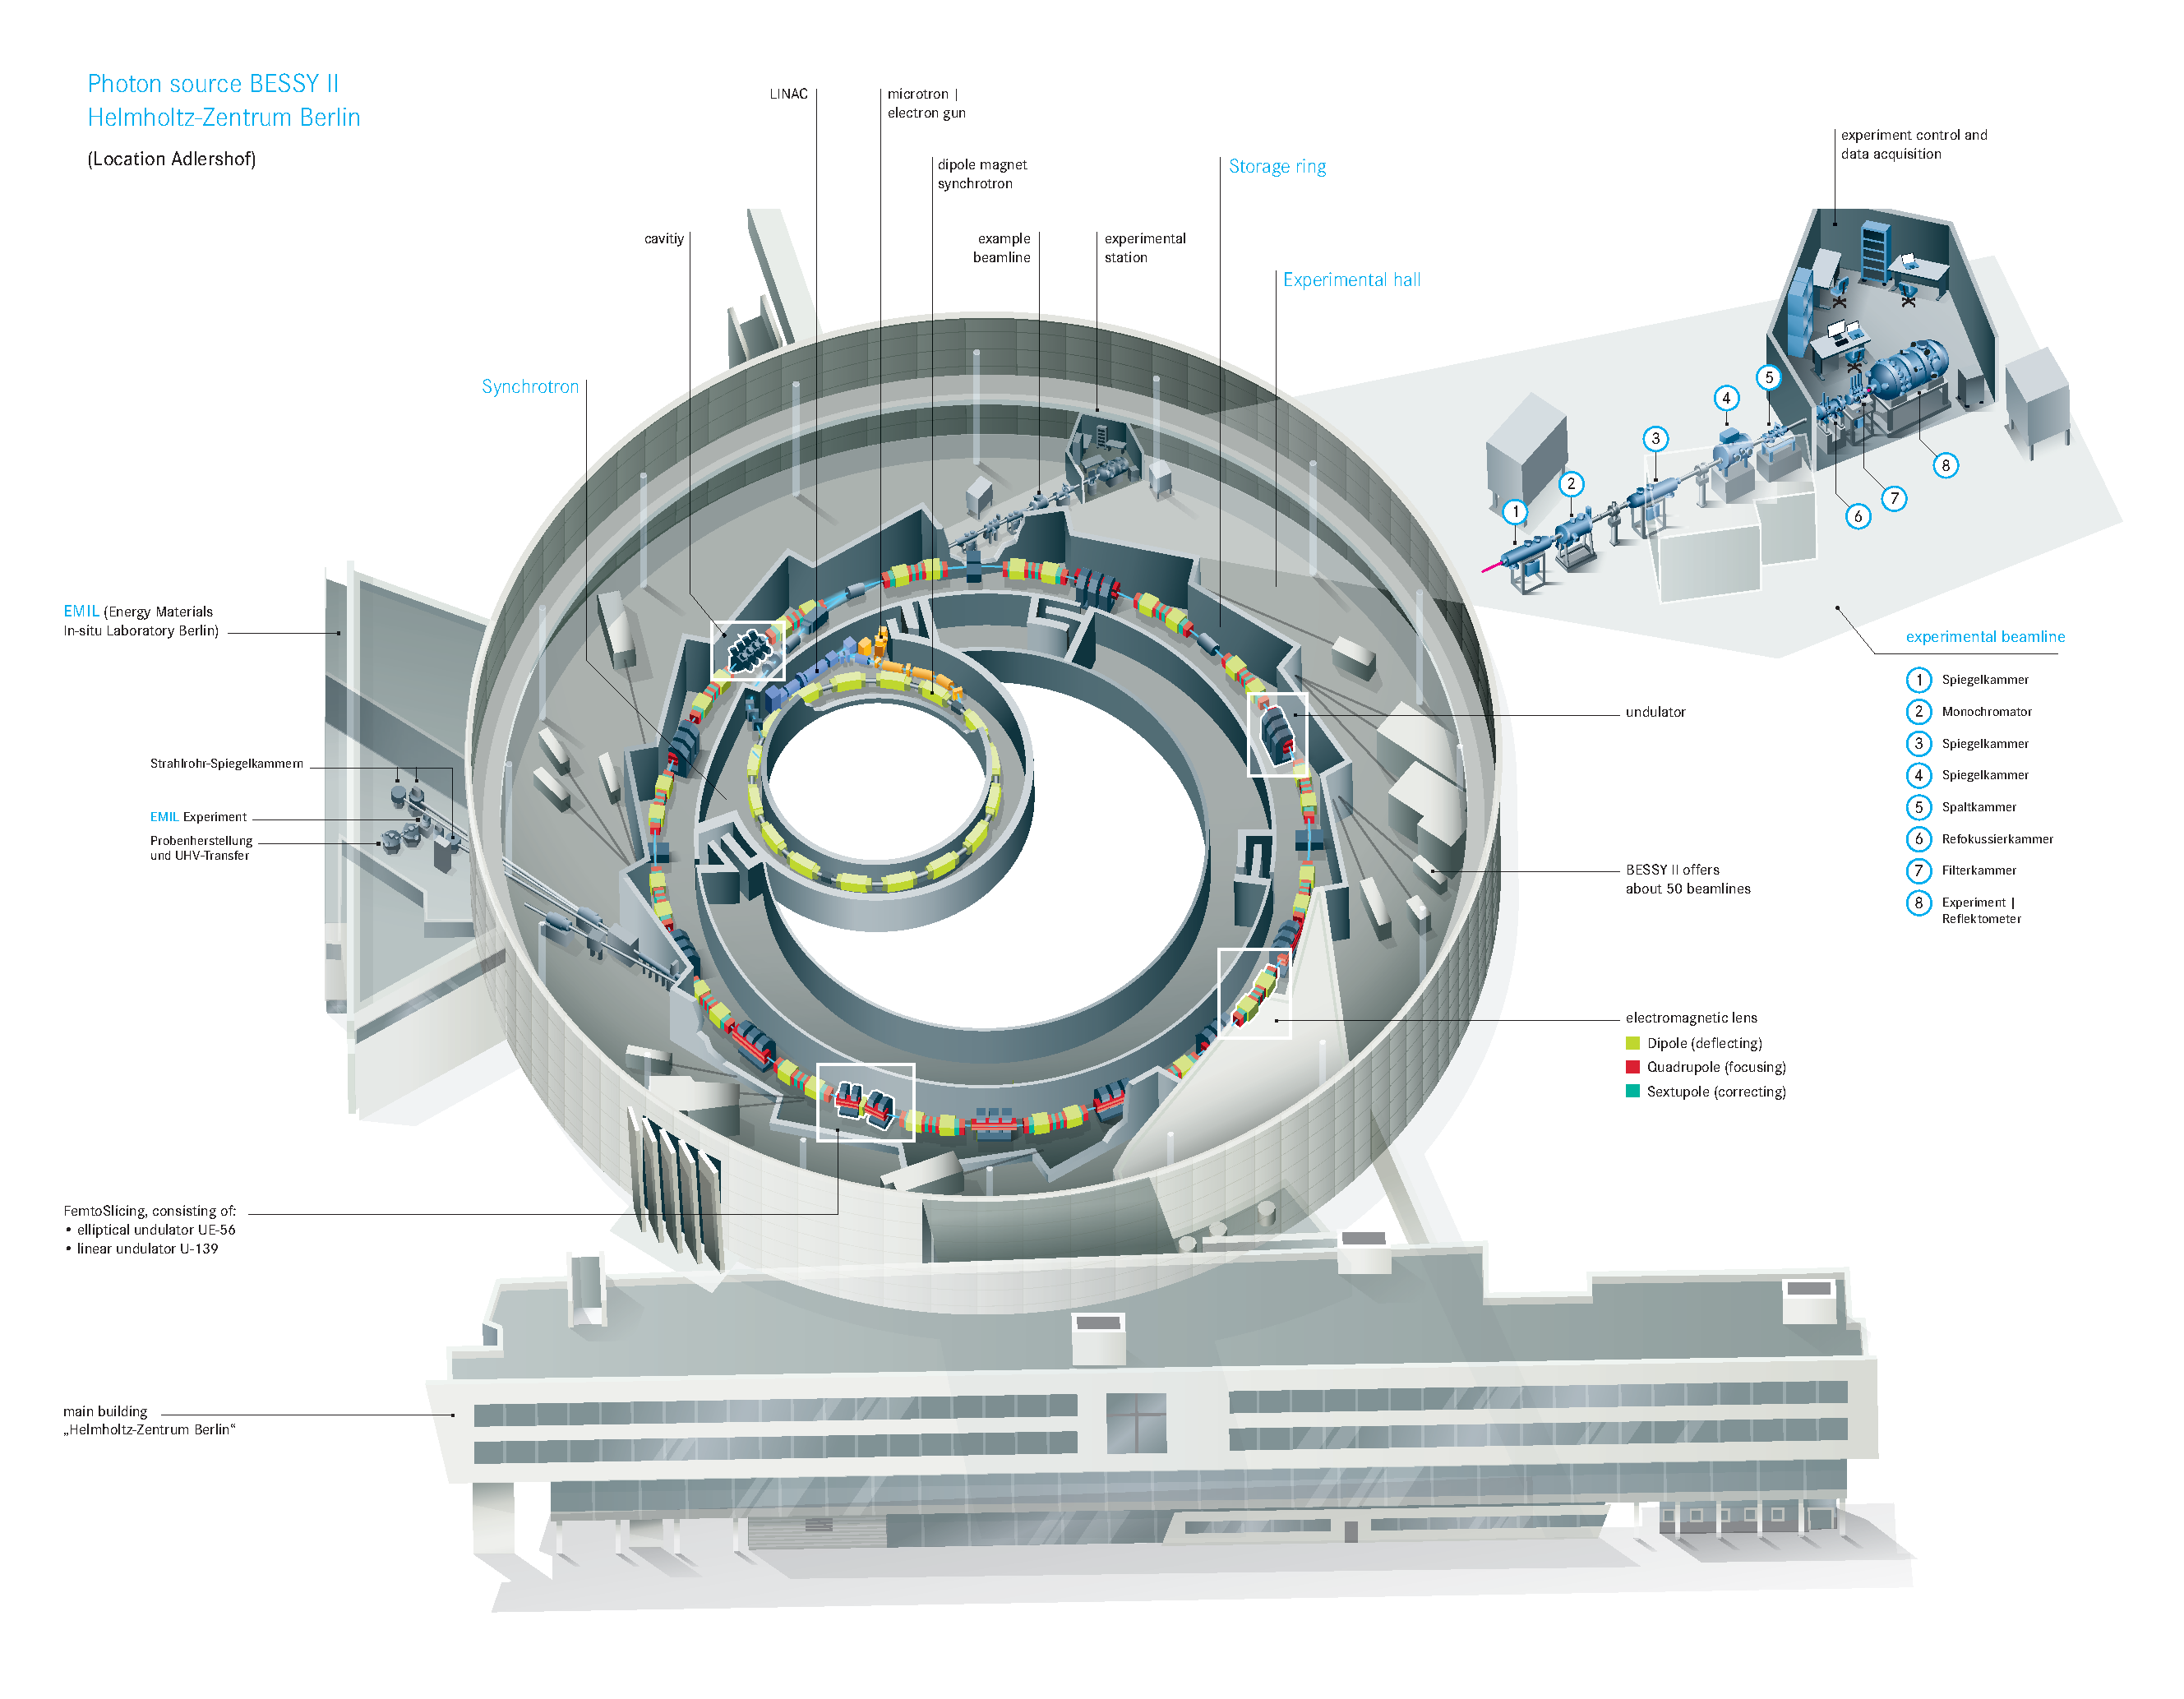
\includegraphics[width=0.9\textwidth,height=1\textheight,keepaspectratio]{img/bessy_acc_web.pdf}
    \caption[BESSY~II facility]{\label{fig:bessy_acc_web} BESSY~II facility (Source:~\cite{web:bessy_homepage})}
\end{sidewaysfigure}

In order to reach an energy of \SI{1.7}{\giga\electronvolt}, the electrons undergo several chained accelerations (see \cref{fig:bessy_acc_web}), namely:
\begin{enumerate}
    \item DC electrons are provided by an electron gun at an energy of \SI{90}{\kilo\electronvolt},
    \item a LINAC (\textbf{lin}ear \textbf{ac}celerator) increases the energy to \SI{50}{\mega\electronvolt},
    \item the booster (a fast rumping synchrotron) accelerate the particles to their full energy of \SI{1.7}{\giga\electronvolt} in not more than \SI{30}{\milli\second}.
\end{enumerate}

When this energy is reached, the electrons are injected to the storage ring, which ensure that the electrons are kept at the same energy.

Another important property of BESSY~II is that it is operated in \textit{top-up mode}. This means that its current must be constant over time (in this case: \SI{300}{\milli\ampere}). However, electrons are likely to collide into each other or with the rest-gas atoms of the vacuum chamber. To achieve the top-up mode and counter the loss of electrons, new injections from the acceleration chain take place approximatively every 2~minutes to repopulate the storage ring.

\section{Motivation}
The most important properties of the synchrotron radiation are its brilliance and brightness, which represent the quality of the beam. The brightness describes the angular divergence of the beam, and the brilliance includes information about its transverse dimension: both are expected to be as small as possible to be in the configuration in which the beam is the most point-like. (See \cref{apx:brightness_brilliance} for the exact definitions).

The main purpose of BESSY~II is to provide a light radiation with high quality brilliance and brightness over time. To achieve this, the light source itself must be very stable and the electron beam very small. The stability of the orbit is required to be well bellow the transverse beam dimensions, which are for BESSY~II storage ring \SI{100}{\micro\meter} in the horizontal direction and \SI{20}{\micro\meter} in the vertical direction.

Therefore, significant attention is drawn to the control of the storage ring orbit: the beam diameter must be as small as possible and therefore always well centered in the vacuum chamber. Although the storage ring is designed to achieve this, perturbations or misalignment in the accelerator optics occur, and must be corrected. Orbit feedback is used here to correct and stabilize the orbit and to keep it focused.

\section{Summary}
BESSY~II is a powerful light source, with a nominal energy of \SI{1.7}{\giga\electronvolt}, that produces a light of high quality, which is a wide spectrum and high brilliance. In order to keep the quality of these properties, removing perturbation sources or correcting the orbit is needed.

In the following, \cref{sec:acc_physics} will provide the needed accelerator physics backgrounds. \Cref{sec:correction} will cover correction methods, first introducing the state of the art in the particle accelerator community, and more specially at BESSY~II. Based on this, the improvement conducted during this work will be described. \Cref{sec:control} will discuss how models and simulations where conducted in order to propose better controllers. In \cref{sec:localization}, algorithms conceived and implemented during this thesis to localize perturbation sources will be presented. Finally \cref{sec:conclusion} will provide an overview of the results achieved with this work and some insights on how to go further.

% !TeX encoding = UTF-8
% !TeX spellcheck = en_US
% !TeX root = ../MasterThesis_OlivierChurlaud_2016.tex

\chapter{Basics of particle accelerator physics}
\label{sec:acc_physics}
In order to be able to localize and correct perturbation, the effects of a perturbation on a particle trajectory must be clearly understood. This section will the particle motion in circular accelerator and define the parameters needed for the following explanations.

The beam trajectory can be studied in various ways. One easier and well used method stems from the field of linear beam optics (by analogy between beam and light focusing and steering). Here will be solely described what is needed in the next sections. A full reference can be found in~\cite{book:wille}. This section is mostly inspired by the chapter 3 of this same reference.

\section{Geometry -- Frame of reference -- Kinematics}
The term \emph{orbit} refers to the ideal trajectory of the particles, which is fixed by the construction of the accelerator.

The frame of reference is $K=(\vec{e}_x,\vec{e}_y, \vec{e}_s)$, which origin follows the beam. $\vec{e}_x$ is the horizontal axis directed towards the exterior of the orbit and normal to its curve, $\vec{e}_y$ is the vertical axis and $\vec{e}_s$ the tangential axis to the orbit.
\begin{figure}
    \centering
    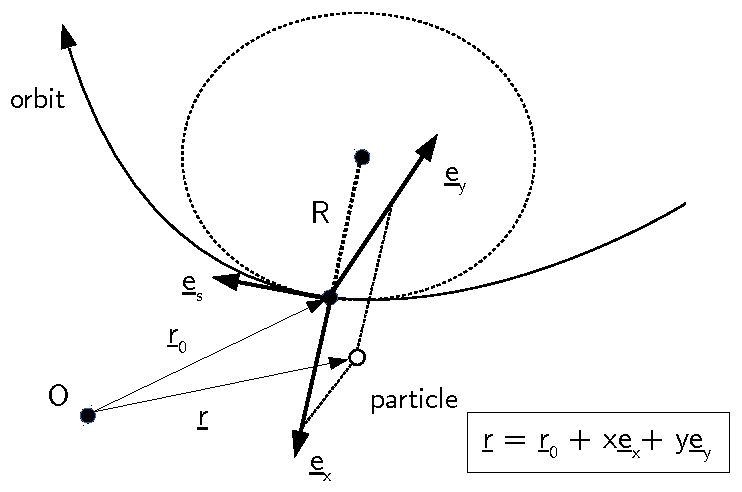
\includegraphics[width=0.8\linewidth]{img/orbit_coordinates.pdf}
    \caption[Description of the co-moving coordinate system]{\label{fig:coordinate system}Description of the co-moving coordinate system (inspired by~\cite{book:wille}, Fig~3.2)}
\end{figure}
Let $\varphi$ be the azimuth angle, oriented by $\vec{e}_y$. Then, since $ds = -R d\varphi$, it can be written
\begin{equation}
\frac{d \varphi}{d t}  = -\frac{1}{R} \frac{d s}{d t}.
\end{equation}

Using the derivation formula of polar coordinate yields
\begin{align}
&\dot{\vec{e}}_x = \frac{d\vec{e}_x}{d t} = -\dot{\varphi} \vec{e}_s = \frac{1}{R} \dot{s}\vec{e}_s \nonumber \\
&\dot{\vec{e}}_y = 0 \\
&\dot{\vec{e}}_s = \frac{d\vec{e}_s}{d t} = \dot{\varphi} \vec{e}_x = -\frac{1}{R} \dot{s}\vec{e}_x \nonumber.
\end{align}

Let $\vec{r} = \vec{r}_0 + x\vec{e}_x + y \vec{e}_y$ be the position of a given particle in a Galilean reference frame (with $\vec{r}_0$ the position of the origin of the moving coordinates, see \cref{fig:coordinate system}) and let $x'$ be the spatial derivative with respect to $s$ so that:
\begin{equation}
\begin{aligned}
&\dot{x}= \frac{dx}{ds}\frac{ds}{dt} = x'\dot{s}  \\
&\ddot{x}= x''\dot{s}^2+x'\ddot{s}.
\end{aligned}
\end{equation}
It follows, after some algebraic manipulations:
\begin{align}
\label{eq:kinematics}
&\vec{r} = \vec{r}_0 + x\vec{e}_x + y \vec{e}_y \nonumber \\
&\dot{\vec{r}}= x' \dot{s} \vec{e}_x + y'\dot{s} \vec{e}_y  + \left(1+\frac{x}{R}\right)\dot{s}\vec{e}_s\\
&\ddot{\vec{r}}= \left[x'' \dot{s}^2 + x' \ddot{s} - \left( 1+\frac{x}{R} \right)\frac{\dot{s}^2}{R}\right] \vec{e}_x + (y''\dot{s}^2 + y'\ddot{s}) \vec{e}_y \nonumber \\
& \hspace{14em} + \left[\frac{2}{R}x'\dot{s}^2 +\left(1+\frac{x}{R}\right)\ddot{s}\right]\vec{e}_s \nonumber
\end{align}

\section{Assumptions}
The following assumptions are assumed to be valid.
\begin{description}
    \item{A1 --} The particles move essentially parallel to $\vec{e}_s$: in the first order
    \begin{equation*}
        \vec{v} = v_s \vec{e}_s.
    \end{equation*}
    \item{A2 --} The magnetic field has only transverse components:
        \begin{equation*}
        \vec{B} = (B_x, B_y, 0).
        \end{equation*}
    \item{A3 --} The electric field is negligible with respect to the magnetic field.
    \item{A4 --} The velocity of the particle varies very slowly in a magnet: $\ddot{s} \approx 0$.
    \item{A5 --} The particles move at relativistic velocities, so the effect of the magnetic field is negligible on longitudinal components: only transverse components will be considered.
    \item{A6 --} The momentum of the particles is $p = p_0+\Delta p$, with the condition $\Delta p \ll p_0$ (which is well satisfied in accelerators).
\end{description}

\section{Equation of motion}
\label{sec:eq_motion}
Newton's second law can be applied with the Lorentz force
\begin{equation}
\dot{\vec{p}} = e(\vec{E}+\vec{v} \times \vec{B})
\end{equation}
which according to (A3) becomes
\begin{equation}
\ddot{\vec{r}} = \frac{e}{m}(\dot{\vec{r}} \times \vec{B})
\end{equation}

According to (A2), the magnetic field is only transversal, which yields
\begin{equation}
\label{eq:lorentz_transv}
\ddot{\vec{r}} = \frac{e}{m}(\dot{\vec{r}} \times \vec{B})
= \frac{e}{m}
    \begin{pmatrix}
        -\left(1+\frac{x}{R}\right)\dot{s}B_y \\
        \left(1+\frac{x}{R}\right)\dot{s}B_x \\
        x'\dot{s}B_y - y'\dot{s}B_x
    \end{pmatrix}.
\end{equation}

Using (A5), the $s$-component does not need to be considered and using (A4) in \cref{eq:kinematics} allows to remove every $\ddot{s}$ factors, so that \cref{eq:lorentz_transv} can be rewritten as
\begin{equation}
\begin{aligned}
x'' \dot{s}^2 - \left(1+\frac{x}{R}\right)\frac{\dot{s}^2}{R}
&= -\frac{e}{m} \left(1+\frac{x}{R}\right)\dot{s}B_y \\
y'' \dot{s}^2 &=    \left(1+\frac{x}{R}\right)\dot{s}B_x.
\end{aligned}
\end{equation}
Finally, because $p=mv$ and using \cref{eq:kinematics} combined with (A1),
\begin{equation}
m = \frac{p}{v} = \frac{p}{\scal{\vec{v}}{\vec{e}_s}} = \frac{p}{\left(1+\frac{x}{R}\right)\dot{s}}
\end{equation}
can be substituted to obtain
\begin{equation}
\begin{aligned}
x''-\left(1+\frac{x}{R}\right)\frac{1}{R} &= -\frac{e}{p} B_y\left(1+\frac{x}{R}\right)^2 \\
y'' &= \frac{e}{p} B_x\left(1+\frac{x}{R}\right)^2
\end{aligned}
\end{equation}

According to (A6), it can be written to first order
\begin{equation*}
\frac{1}{p} = \frac{1}{p_0} \left(1-\frac{\Delta p}{p_0}\right).
\end{equation*}

Furthermore the magnetic field can be approximated to first order with:
\begin{equation}
\frac{e}{p_0} B_y = \frac{1}{R}-kx \qquad\qquad \frac{e}{p_0} B_x = -ky
\end{equation}
which yields
\begin{equation}
\begin{aligned}
x''-\left(1+\frac{x}{R}\right)\frac{1}{R} &= -\left(\frac{1}{R}-kx\right)\left(1-\frac{\Delta p}{p_0}\right)\left(1+\frac{x}{R}\right)^2 \\
y'' &= -ky\left(1-\frac{\Delta p}{p_0}\right)\left(1+\frac{x}{R}\right)^2
\end{aligned}
\end{equation}

Finally removing terms of second order ($\frac{x}{R} \ll 1$, $\frac{\Delta p}{p_0} \ll 1$) leads to the linear equations of motion in a magnetic structure:

\begin{empheq}[box=\fbox]{equation}
\label{eq:motion_particle}
\begin{aligned}
x''(s) + \left(\frac{1}{R^2(s)} - k(s)\right) x(s) &= \frac{1}{R(s)}\frac{\Delta p}{p_0} \\
y''(s) + k(s) y(s) &= 0
\end{aligned}
\end{empheq}

\section{Beta function and betatron oscillation}
\label{sec:beta_func}
The beta function will provide a description of properties of a beam of many particles.

The only further assumption is that $\frac{1}{R} = 0$ and $\frac{\Delta p}{p_0}=0$. The orbit curve is thus assumed almost flat and the momentum deviation negligible. \Cref{eq:motion_particle} turns in Hill's differential equation:
\begin{equation}
\label{eq:hill_diff}
	x''(s) - k(s) x(s) = 0
\end{equation}
which solution is the transverse oscillation of the orbit, or \emph{betatron oscillation}
\begin{equation}
\label{eq:hill_sol_cst}
x(s) = A u(s) \cos \left(\Psi(s)+\phi \right).
\end{equation}

The phase and the amplitude depend of the position $s$; $A$ and $\phi$ being integration constants.

Inserting \cref{eq:hill_sol_cst} in \eqref{eq:hill_diff} it follows
\begin{equation}
A\left[u''- u \Psi'^2 - k u \right] \cos\left(\Psi+\phi\right) - A\left[2u'\Psi'+u\Psi''\right]\sin\left(\Psi+\phi\right) = 0.
\end{equation}

$A \ne 0$ and $\Psi(s)$ having different values for every $s$, the previous equation provides two conditions
\begin{align}
u''- u \Psi'^2 - k u = 0 \label{eq:hill_cond1}\\
2u'\Psi'+u\Psi'' = 0 \label{eq:hill_cond2}.
\end{align}

\Cref{eq:hill_cond2} leads to
\begin{equation}
2\frac{u'}{u} + \frac{\Psi''}{\Psi'} = 0
\end{equation}
which can be integrated as
\begin{equation}
\label{eq:phase_psi}
\Psi(s) = \int \limits_{0}^{s} \frac{d\sigma}{u^2(\sigma)}.
\end{equation}

The \emph{beta function} $\beta(s)$ is defined as
\begin{equation}
\label{eq:beta_func}
\beta(s) := u^2(s).
\end{equation}
and allows to rewrite
Substituting $A = \sqrt{\varepsilon}$ provides the final trajectory equation
\begin{empheq}[box=\fbox]{equation}
	\label{eq:orbit_equation}
	x(s) = \sqrt{\varepsilon \beta(s)} \cos\left(\Psi(s)+\phi \right)
\end{empheq}

The constant $\varepsilon$ is termed \emph{emittance} and the envelop of the orbit at each position $s$ is $E(s) = \sqrt{\varepsilon \beta(s)}$, which defines the size of the beam.

Finally, deriving $x(s)$ leads to
\begin{align}
    x'(s) &= \frac{\sqrt{\varepsilon \beta'(s)}}{2\sqrt{\beta(s)}} \cos \left( \Psi(s) + \phi \right)
         - \sqrt{\varepsilon \beta(s)}\frac{1}{\beta(s)} \sin \left(\Psi(s)+\phi \right) \nonumber \\
          &= -\sqrt{\frac{\varepsilon}{\beta(s)}} \left[\alpha(s) \cos \left( \Psi(s) + \phi \right)
             + \sin \left(\Psi(s)+\phi \right) \right]
\end{align}
with
\begin{equation}
    \alpha(s) := -\frac{\beta'(s)}{2}
\end{equation}

Since the beta function controls the size of the beam, this is the function that must be finely controlled. A matrix calculation method is presented in \cite{book:wille} in order to calculate $\beta(s)$ and $\alpha(s)$ step by step around the orbit. Once these are known, the particle trajectory can be easily calculated through the matrix multiplication
\begin{equation}
\begin{pmatrix}x(s) \\ x'(s) \end{pmatrix} = \mat{M} \begin{pmatrix}x(0) \\ x'(0) \end{pmatrix}.
\end{equation}
From the equations of $x(s)$ and $x'(s)$, some trigonometrical manipulations and choosing $\phi(0)=0$ it can be shown that (with simplified notations)
\begin{equation}
\label{eq:motion_transfert_matrix}
\mat{M} = \begin{pmatrix}
                \sqrt{\dfrac{\beta}{\beta_0}}\left( \cos \Psi + \alpha_0 \sin \Psi  \right)
              & \sqrt{\beta\beta_0}\sin \Psi
             \\ \dfrac{( \alpha_0-\alpha ) \cos \Psi - (1+\alpha_0\alpha)\sin \Psi}{\sqrt{\beta\beta_0}}
              & \sqrt{\dfrac{\beta_0}{\beta}}\left( \cos \Psi-\alpha \sin \Psi \right)
          \end{pmatrix}.
\end{equation}


The two functions $\Psi$ and $\beta$ will be extensively used in the next sections as the perturbation localization process and several correction methods rely on them.

\remark The calculation done for the $x$ direction can be done similarly for the $y$ one, which defines a $\beta_x(s)$, $\beta_y(s)$, $\varepsilon_x$, $\varepsilon_y$, $\Psi_x(s)$ and $\Psi_y(s)$

\section{Tune}
In circular accelerator, the particle undergo periodically the same magnetic fields and therefore the same force. This can lead the amplitude of the beam transverse oscillation to increase, risking to lose the particles in the vacuum chamber walls. This phenomenon is called optical resonance and must be avoided.

As exposed in \cref{sec:eq_motion,sec:beta_func}, if $\frac{\Delta p}{p_0} = 0$ and $K(s)=\frac{1}{R(s)}-k(s)$, the trajectory is given by
\begin{equation}
x''(s)+K(s) x(s) = 0.
\end{equation}

Since $K(s)$ is periodic with the circumference $L$ of the ring, then the trajectory is again (according to Floquet's theorem)
\begin{equation}
x(s) = \sqrt{\varepsilon \beta(s)} \cos\left(\Psi(s)+\Phi\right)
\end{equation}
with $\beta(s)$ periodic of period $L$ as well. The resonant behavior depending on the betatron phase $\Delta \Psi = \Psi(s+L)-\Psi(s)$, the tune $Q$ of the accelerator is defined as
\begin{equation}
\label{eq:tune}
Q = \frac{\Delta \Psi}{2 \pi} = \frac{1}{2 \pi} \oint\frac{ds}{\beta(s)}.
\end{equation}

The tune is a constant for a circular accelerator: it describes the \emph{number of betatron oscillation} undergone by a particle per revolution.

It can be shown that tune values that satisfy
\begin{equation}
\label{eq:coupled_resonance}
m Q_x + n Q_y = p \qquad (m, n, p) \in \mathbb{Z}
\end{equation}
produce coupled resonance of order $|m|+|n|$. A pair of value $(Q_x,Q_y)$ is used as working point so that it either does not satisfy \cref{eq:coupled_resonance} or with a high order (above the 5th order for instance).

\section{Summary}
Two very important functions were defined here: $\beta (s)$ and $\Psi (s)$, respectively the variation of the trajectory amplitude and the betatron phase. These functions highly depend on the accelerator optic and when determined, knowing the real objects that produce them (e.g. magnets, coils) is no more needed.

The tune $Q$ is a constant parameter defined as the number of betatron oscillation per revolution.

The following sections will rely on these three variables as they fully represent the orbit and its variations.

% !TeX encoding = UTF-8
% !TeX spellcheck = en_US
% !TeX root = ../MasterThesis_OlivierChurlaud_2016.tex
\tikzset{
	block/.style = {draw, fill=white, rectangle, minimum height=3em, minimum width=4em},
	gain/.style = {draw, fill=white, isosceles triangle, minimum height=3em, minimum width=2em},
	operator/.style= {draw, fill=white, circle},
	input/.style = {coordinate},
	output/.style= {coordinate},
	pinstyle/.style = {pin edge={to-,thin,black}},
}

\chapter{Orbit correction}
\label{sec:correction}

\section{Motivation}
The accelerators are designed so that the particles follow a given path, which is defined in the case of synchrotrons by the successive bending involved by dipole magnets. Quadrupole magnets are additionally needed to provide focusing and guarantee the closing of the orbit. As the precision of the positioning of the magnets is limited, some errors may destabilize the orbit and increase the deviation of the particles around the theoretical orbit.

In addition, the environment produces perturbations: for instance the 50~Hz of the main power, some not perfectly isolated magnetic sources (like the booster at \SI{10}{\hertz}). \Cref{fig:fft_no_correction} shows the spectrum of the beam displacement from the reference orbit before correction. 
\begin{figure}
	\centering
	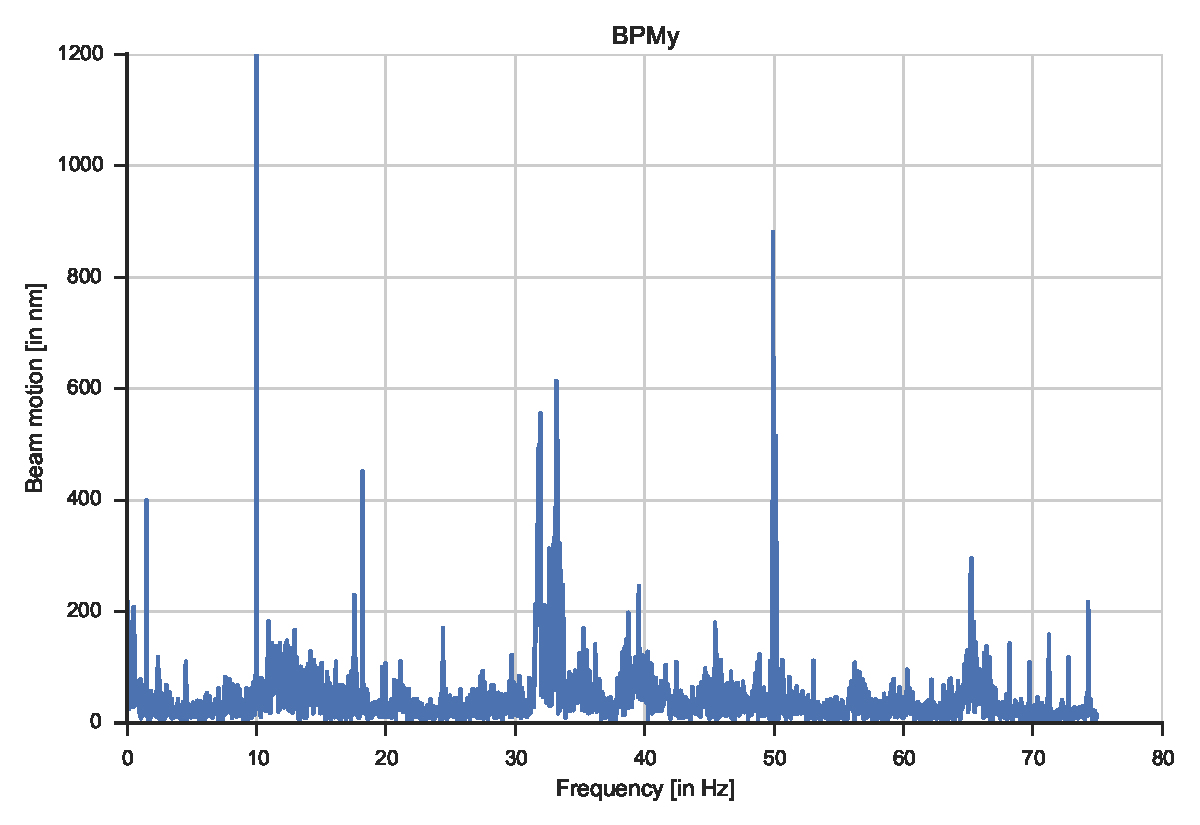
\includegraphics[width=.9\linewidth]{img/fft_no_corr}
	\caption{\label{fig:fft_no_correction} Spectrum of the beam motion, without correction (vertical)}
\end{figure}

In order not to lose electrons in the walls of the vacuum chamber but also to increase the brightness of the synchrotron radiations (and therefore to have focused electron beams), all these residual misalignment and magnetic field errors must be corrected.

The most classical correction methods will be presented here, before explicitly describing the case of BESSY~II and the ameliorations proposed during this thesis.

\section{Monitoring and correction instruments}
To be able to correct the orbit or localize perturbations, some tools must be employed.

\subsection{Beam Position Monitors}
The position of the beam in a given direction is monitored with beam position monitors (BPM).

Several types of BPMs exist, but the important characteristics of the one used at BESSY~II are that they provide a method
\begin{itemize}
	\item which is non invasive (it does not affect the beam or negligibly)
	\item which outputs an electric signal proportional to the distance of the beam from an arbitrary point.
\end{itemize}

This last property means that the measured value must always be subtracted by a reference value.

The raw values output by the BPMs are thus never considered and every orbit position value given (also called BPM value by misuse of language) is always, at position~$s$ and time~$t$
\begin{equation}
\Delta x_\text{BPM}(s,t) = x_\text{BPM}(s,t) - x_\text{BPM,ref}(s)
\end{equation}

\subsection{Correctors}
To correct the orbit, BESSY~II uses dipole magnets, also called corrector magnets (CM) positioned around the storage ring. Each dipole contributes to correcting in a given direction, at a specific position.

\subsection{Monitor and corrector numbers}
The number of monitors and correctors is quite important. Because the correction method used is based on an inversion problem (see \cref{sec:response_matrix}), it is important to have an over-constrained problem. Else a perfect correction would be reached at monitor positions but unconstrained (and thus potentially arbitrary bad) elsewhere.

Therefore the number of BPMs is chosen quite greater than the number correctors.

At BESSY~II there are
\begin{itemize}
	\item 128~BPMs, measuring both horizontal ($\text{BPM}_\text{x}$) and vertical ($\text{BPM}_\text{y}$) direction,
	\item 48~CMs for the horizontal direction ($\text{CM}_\text{x}$) and 64 for the vertical one ($\text{CM}_\text{y}$).
\end{itemize}

\section{Some documented methods}
Several global corrections methods are well documented in the literature. Local orbit bumps (presented in \cref{sec:orbit_bump}) allow local correction and are used to change the path of the orbit (during the injection time for example). The most common ones are the best corrector method and the response matrix method (see \cref{sec:most_effective_corr,sec:response_matrix}), as they provide a global correction, over the whole orbit.

\subsection{Local orbit bumps}
\label{sec:orbit_bump}
Using local orbit bumps is a basic method that gives total control on the orbit local modification to the operator.

\subsubsection{Principle}
Adding a simple dipole on the path of a particle will bring it closer or push it away. As the particles must eventually return to the planned orbit, a series of dipoles can be set one after the other to design an arbitrary path. \Cref{fig:local_bump} shows a minimal example, where the black points represent the magnets, and the dashed line the original orbit. Each magnet $M_i$ has position $s_i$, where the phase is $\Psi_i$ and the beta function  $\beta_i$. The orbit motion at this position is described by the vector $\vec{x}_i = (x_i , x'_i)$.
\begin{figure}
	\centering
	\begin{tikzpicture}[auto, node distance=1.2,>=latex']
	%\draw[help lines, yellow] (-1,-4)grid(15,3);
	% We start by placing the blocks
	\coordinate [] (lleft) {};
    \coordinate [right=.2 of lleft] (origin) {};
    \coordinate [below=.2  of origin] (xaxisbottom) {};
    \coordinate [above=2 of origin] (xaxistop) {};
	\node [draw, circle, fill=black, right=2 of lleft, label=below:$M_1$] (leftm) {};
    \node [draw, circle, fill=black, right=3 of leftm, label=below:$M_2$] (middlem) {};
	\coordinate [above=1.5 of middlem] (topcoord) {};
	\node [draw, circle, fill=black, right=4 of middlem, label=below:$M_3$] (rightm) {};
	\coordinate [right=2 of rightm] (rright) {};
	% Once the nodes are placed, connecting them is easy.
	\draw [-] (lleft) -- (leftm);
	\draw [-] (leftm) to [bend left=35] (topcoord);
	\draw [-] (topcoord) to [bend left=35] (rightm);
	\draw [->] (rightm) -- node [near end] {$s$} (rright);
    \draw [->] (xaxisbottom)  -- node [near end]{$x$} (xaxistop);
   	\draw [dashed] (leftm) -- (rightm);
	\end{tikzpicture}
	\caption{\label{fig:local_bump}Local bump with 3 magnets (inspired by~\cite{book:wille}, Fig~3.47)}
\end{figure}

The strengths $\kappa_1$, $\kappa_2$, $\kappa_3$ of each magnets can be calculated with the formalism introduced in \cref{sec:beta_func}, \cref{eq:motion_transfert_matrix} in order to achieve the right displacement and respect the closed orbit condition. The following conditions must be fulfilled (closed orbit):
\begin{equation}
\vec{x}_1 = \dbinom{0}{\kappa_1} \qquad \text{and} \qquad
\vec{x}_3 = \dbinom{0}{-\kappa_3}
\end{equation}

The orbit motion at $s_3$ is the superposition of the effects of $M_1$ and $M_2$ alone. It can thus be written
\begin{equation}
\vec{x}_3 = \mat{M}_{1 \rightarrow 3} \vec{x}_1 + \mat{M}_{2 \rightarrow 3} \dbinom{0}{\kappa_2}
\end{equation}
or
\begin{equation*}
\begin{pmatrix} 0 \\ -\kappa_3 \end{pmatrix} =
\begin{pmatrix} a_{11} & a_{12} \\ a_{21} & a_{22} \end{pmatrix} \begin{pmatrix} 0 \\ \kappa_1 \end{pmatrix} +
\begin{pmatrix} b_{11} & b_{12} \\ b_{21} & b_{22} \end{pmatrix} \begin{pmatrix} 0 \\ \kappa_2 \end{pmatrix}
\end{equation*}
Solving this system of equations and replacing the coefficients of the matrix by their expression in \cref{eq:motion_transfert_matrix} leads to the values of $\kappa_2$ and $\kappa_3$ in function of $\kappa_1$ (see \cite{book:wille}, p.130 for the exact equations). This can allow an arbitrary displacement of the orbit at a given position. This can be extended to a version with $N$ magnets, which allows the free setting of $N-2$ parameters ($x$ or $x'$). This is extensively described in \cite{book:wille}.

\subsubsection{In practice}
This solution is used for instance to shift a part of the orbit during particle injections, in order not to disturb already stored particles. It can also be used to counter a known localized perturbation which source cannot be removed.

It is indeed very efficient to locally shift the orbit. However it cannot be used for correction, as it only modify the path of the orbit itself and only locally.

\subsection{Most effective corrector method}
\label{sec:most_effective_corr}
This method is based on the fact that orbit shifts are often caused by strong localized disturbances. Its goal is to correct particularly each disturbance.

\subsubsection{Principle}
Given a distorted orbit, the optimal gain for each corrector is calculated by a mean square error algorithm (see \cref{eq:gain_bestcorr} and \cite{book:wille}). The corrector which provides the best correction is selected: it is the most effective corrector.

Let's assume that the $i$th corrector, at position $s_i$, has the optical parameters $\beta_i$, $\alpha_i$ and $\Psi_i$, and that $m$ monitors are set around the orbit with parameters $\beta_j$, $\alpha_j$ and $\Psi_j$, and read a displacement $u_j$ from the reference orbit ($1 \leq j \leq m$).

The strength $\kappa_i$ of the field at the position $s_i$ is obtained minimizing the function
\begin{equation}
	\label{eq:gain_bestcorr}
    f_i(\kappa_i) = \sum\limits_{j=1}^{m} (u_j-x_{ij}(\kappa_i))^2
                  = \sum\limits_{j=1}^{m} (u_j- \kappa_i h_{ij})^2
\end{equation}

with, if $\Delta \Psi_{ij} := \Psi_j-\Psi_i$,

\begin{align}
    \label{eq:hij}
    x_{ij}(\kappa_i) &= \kappa_i h_{ij} \nonumber\\
                     &= \kappa_i \frac{\sqrt{\beta_i \beta_j}}{2}
                         \left[
                             \frac{\cos(\Delta \Psi_{ij}) - 2\alpha_i \sin(\Delta\Psi_{ij})}
                                  {\tan (\pi Q)} + \sin (\Delta\Psi_{ij})
                         \right].
\end{align}

It follows that
\begin{equation}
    \kappa_i = \frac{\sum\limits_{j=1}^m u_j h_{ij}}{\sum\limits_{j=1}^m h_{ij}^2}
\end{equation}

The $i$th corrector is attributed the gain $-\kappa_i$ to compensate the field.

\subsubsection{Iterative version}
When the most effective corrector is found, the process is reiterated on the corrected orbit with the remaining correctors. By doing this until all corrector are used (or that adding a correction does not improve the orbit) a comprehensive correction is reached.

\subsubsection{Practical issue}
The problem of this method is that each corrector must be tested once, and this for each iteration: the initialization of the correction is long and is then fixed. Moreover, the correction is less efficient than the other ones presented here~\cite{book:wille}.

\subsection{Response matrix}
\label{sec:response_matrix}
This section is mainly based on~\cite{book:wille}, \cite{art:decker-1991} and \cite{art:plouviez-1999}.

\subsubsection{Inverse problem}
This correction is based on solving the following inverse problem: the expected orbit being known, how to set the correctors in order to achieve it? To solve it, the response matrix $\mat{S}$ is introduced.

The response matrix $\mat{S}$ is defined by the equation $\vec{X} = \mat{S}\, \vec{\Theta}$ where $\vec{\Theta}$ is the \emph{kick vector} (i.e. the vector of strength of the field generated by each corrector) and $\vec{X}$ the vector of \emph{orbit change}. If the accelerator has $M$ monitors and $N$ correctors, then $\mat{S}$ is a $M \times N$ matrix. $\mat{S}$ is often termed \emph{forward} or \emph{observation matrix} because it describes the effects of a given phenomenon. Indeed, each coefficient $S_{ij}$ of the matrix is the orbit change at the position $s_i$ (of the $i$th monitor), for a kick of unity 1 at the position $s_j$ (of the $j$th corrector).

Inversing the response matrix will provide the correction to apply. Since it's very common to have more monitors than correctors, the matrix is not square. A \emph{singular value decomposition} (SVD) is used on the matrix to provide a pseudo-inversion $\mat{S}^*$ of $\mat{S}$.

Using the SVD also allows to use only the most significant singular values in the correction. This prevents to over-correct the orbit, by not considering less significant values that can result of noise in the monitors during the measure, numerical artifacts or incorrections in the response matrix.

The correction can then be performed
\begin{equation}
\vec{\Theta} = \mat{S}^* \vec{X}.
\end{equation}

\subsubsection{Acquisition of the response matrix}
Before solving the inverse problem, the response matrix must first be determined. This can be achieved in two different ways: by describing the magnet structure and explicitly calculating the matrix or by acquiring it in an experimental way.

\paragraph{Calculation of the response matrix}
The matrix can be theoretically calculated by using the accelerator model and physics. This was already used in \cref{sec:most_effective_corr} and using the same calculations leads to setting, for the $i$th monitor and $j$th corrector,
\begin{equation}
S_{ij} = h_{ij}
\end{equation}
with $h_{ij}$ as defined in \cref{eq:hij}.

The main flaw of this method is that it is only a model which hence may not exactly represent the reality. Some misalignments of magnets or external magnetic perturbations would not be taken in account. It's however a good first approach.

\paragraph{Experimental acquisition of the response matrix}
A more common and precise way of constructing the response matrix is empirical: it suffices to give a unitary value to a corrector and to read the monitors to obtain a column $\mat{S}$. Doing so for each corrector provides the whole matrix.


\section{State of the art at BESSY II}
\label{sec:correction_state_of_art}
BESSY II currently implements a Fast Orbit Feedback (FOFB) which is based on the response matrix inverse. The correction algorithm will be first described in \cref{sec:correction_sa_corr}, and current choices will be discussed by references found in literature. A technical overview will then be provided in \cref{sec:correction_sa_technical}, presenting the actual processes taking part in the correction.

\subsection{The correction}
\label{sec:correction_sa_corr}
Using the response matrix to correct the orbit is quite common \cite{book:wille,art:plouviez-1999,art:li-2001}. However, as already highlighted in \cref{sec:response_matrix}, the matrix never perfectly represents the orbit and because of noises in the environment, it is not sufficient. In general only the largest singular values are used and some corrections are additionally needed in the frequency domain.

To cope with these additional requirements, a PID correction (proportional response with gain $K_p$, integral response with gain $K_i$ and derivative response with gain $K_d$) is used at BESSY~II. It also deals with the delays introduced by the process between the time the orbit is read by the BPMs and the moment the correction is actually applied \cite{art:plouviez-1999}.

The full process goes as presented in \cref{fig:block_correction}.

\begin{figure}
    \centering
    \begin{tikzpicture}[auto, node distance=1.2,>=latex']
    %\draw[help lines, yellow] (-1,-4)grid(15,3);
        % We start by placing the blocks
        \node [operator] (sum) {$+$};
        \node [input, above=2 of sum.center] (xref) {};
        \node [operator, right=of sum] (prod) {$\times$};
        \node [input, above=2 of prod.center] (invS) {};
        \node [gain, right=0.7 of prod] (gain) {$\vec{W}$};
        \node [block, right=of gain] (PID) {~PID~~};
        \node [input, above=2 of PID.center] (pidcoef) {};
        \node [operator, right= of PID] (sum2) {$+$};
        \node [block, above right= 0.8 and 0.65 of sum2.center] (delay) {Delay T};
        \coordinate [right=3 of sum2.center] (straight) {};
        \node [draw, ellipse, minimum height=1.7cm, minimum width=5.5cm, below=1 of straight] (ring) {Storage Ring};
        \node [draw, ellipse, line width=1pt, dotted, minimum height=.5cm, minimum width=.8cm, above=-.25 of ring.north, label=above right:\footnotesize Correctors] () {};
        \node [draw, ellipse, line width=1pt, dotted, minimum height=.5cm, minimum width=.8cm, above=-.25 of ring.west, label=above left:\footnotesize BPMs] (BPM) {};
        \coordinate [left=1 of sum.center](leftback) {};

        % Once the nodes are placed, connecting them is easy.
        \draw [->] (xref)     -- node [pos=0.85, left]{$-$} node {$\vec{X}_\text{ref}$}(sum);
        \draw [->] (sum)      -- node {$\Delta\vec{X}$} (prod);
        \draw [->] (invS)     -- node {$\mat{S}^*$}        (prod);
        \draw [->] (prod)     -- node {}             (gain);
        \draw [->] (gain)     -- node {$\Delta\vec{\Theta}_\text{t}$}             (PID);
        \draw [->] (PID)      -- node {$\Delta\vec{\Theta}$} node[pos=0.80, below] {$-$}      (sum2);
        \draw [->] (pidcoef)  -- node[pos=0.70, above, fill=white] {PID coeff.} (PID);
        \draw [-]  (sum2)     -- node {}  (straight);
        \draw [->] (straight) |- node[pos=0, right] {$\vec{\Theta}_{(n)}$} (delay);
        \draw [->] (delay)    -| node[above] {$\vec{\Theta}_{(n-1)}$} (sum2);
        \draw [->] (straight) -- node[pos=0.80] {}  (ring);
        \draw [-]  (ring)     -| node {}             (leftback);
        \draw [->] (leftback) |- node[pos=0.5] {$\vec{X} $}  (sum.west);
\end{tikzpicture}
    \caption{\label{fig:block_correction}The correction process used at BESSY~II}
\end{figure}

The control value at correction cycle $n$ is the differential orbit
\begin{equation}
 \Delta \vec{X}[n] := \vec{X}[n]-\vec{X}_\text{ref}
\end{equation}
which is expected to be close to 0. The correction provided by the weighted response matrix is then processed
\begin{equation}
\Delta \vec{\Theta}_\text{t}[n] :=  \left(\mat{S}^{-1} \cdot \Delta \vec{X}[n] \right) \odot \vec{W}
\end{equation}
(with $\odot$ the point-wise multiplication and $\vec{W}$ the vector of weights) and modulated by the PID correction. The ideal PID in the Laplace form is described with
\begin{equation}
H_{PID}(s) = K_p + \frac{K_i}{s} + K_d \cdot s
\end{equation}
or, with the z transform (calculated with Euler's method),
\begin{equation}
H_{PID}(z) = K_p + \frac{K_i}{1-z} + K_d \cdot (1-z)
\end{equation}
which yields
\begin{equation}
\Delta \vec{\Theta}[n] =  K_p \cdot \Delta \vec{\Theta}_\text{t}[n] + K_i \cdot \sum\limits_{k=0}^{n-1}\Delta \vec{\Theta}_\text{t}[k] + K_d \cdot \left(\Delta \vec{\Theta}_\text{t}[n] - \Delta \vec{\Theta}_\text{t}[n-1]\right).
\end{equation}

The real correction is eventually the accumulation of all corrections
\begin{equation}
\vec{\Theta}(n) = \vec{\Theta}[n-1] - \Delta \vec{\Theta}[n].
\end{equation}

For stability reasons, the PID was always implemented as a pure proportional corrector ($K_i$ and $K_d$ being set to zero). Indeed, because of the last accumulation, it was of course behaving like a proportional integrator (PI), which forbade the use of the other coefficients in the PID correction. In the simulations described in \cref{sec:correction_simulation}, a corrector PID can be implemented with more optimal coefficients. It is however important that the correction starts from an initial value known to be stable, so that the beam stays focused.

\subsection{Technical overview}
\label{sec:correction_sa_technical}
The correction is naturally automatized. Because the read/write actions should be really fast, a specific infrastructure was designed. This is represented on \cref{fig:cbox_mbox}.

\begin{figure}[!h]
    \centering
    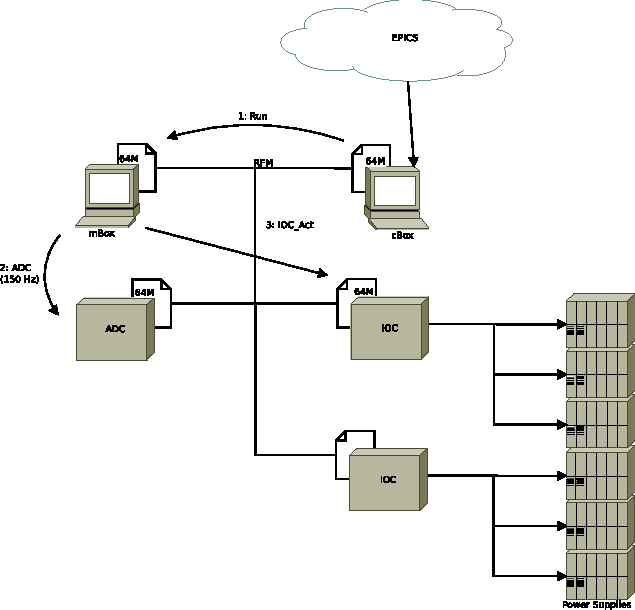
\includegraphics[width=.85\linewidth]{img/mBox_cBox}
    \caption{\label{fig:cbox_mbox}cBox and mBox: the correction infrastructure at BESSY~II}
\end{figure}

All elements are connected to a reflective memory (RFM), which provides a high speed and low latency interface. This memory space is split in specified divisions to prevent data collisions: one part contains the configuration, a second the orbit values and the last one the correction values.

\paragraph{Actors}
The following actors are playing a role in the process:
\begin{itemize}
    \item the \textbf{analog-to-digital converter (ADC)} reads the orbit displacement values from the BPMs and makes them available to the other actors.
    \item the \textbf{cBox} controls (= \textit{c}) the correction. It defines when to read the values of the BPMs and when to write the new correction values, it provides initializations values. The operators are communicating with this process to configure the correction.
    \item the \textbf{mBox} does the math (= \textit{m}) of the correction. When allowed by the cBox, it reads the BPMs values, do the maths to define the new correction values (multiplication with the response matrix, PID correction) and write them to the communication bus. This process also publish the values it reads and writes so that client programs can subscribe to this data stream and reuse the values internally.
    \item the \textbf{input-output controllers (IOCs)} write the correction values to the power supplies commands when they are available.
    \item the \textbf{power supplies (PS)} provide a given power to the corrector magnets.
\end{itemize}

\paragraph{Process description}
After having received the authorization to run from the cBox, the mBox process starts. It first does its full initialization, which only happens on start (the response matrix, the reference orbit, the PID parameters, etc. cannot change while the mBox process is running), and starts the ADC. From this time, the ADC will write new orbit values to the RFM at a rate of \SI{150}{\hertz}.

The mBox waits for the ADC interruption to read the new orbit data from the RFM. The correction is then calculated (in Amperes) and the values are converted in the DAC input format (basically unsigned integers). This data is written back to RFM and an interruption is sent to inform the other elements that the new values are available. This is read by the IOCs that relay to the power supplies alimenting the corrector magnets.

This defines a real time process, repeated at the frequency of \SI{150}{\hertz}.

The duration of each step is as following:
\begin{itemize}
\item orbit value acquisition (BPMs): 0.3 to \SI{1.7}{\milli\second}
\item correction computation: 0.5 to \SI{1}{\milli\second}
\item writing the correction to the RFM: 0.5 to \SI{1}{\milli\second}
\end{itemize}

\remark One of the side works done during this thesis was rewriting the whole mBox in C++ in a very object oriented way to allow a smaller computation time (the original one was written in \textsc{Matlab}), easier improvement and feature additions (like a dynamic correction, easier communication with external scripts, production/experimental modes, etc.). This is fully presented in \cref{apx:mbox}.

\subsection{Result overview}
The results of this correction can be seen on \cref{fig:compare_fofb}: the low frequencies and most of the peaks are reduced, which is a real gain for the end users of the accelerator. Unfortunately, the correction gain provides only a correction up to $\sim\!\SI{12}{\hertz}$., and increasing it let the system become instable. Such a correction is therefore not always sufficient and other methods are experimented to decrease the remaining disturbances.

\begin{figure}
    \centering
    \begin{subfigure}[b]{0.8\textwidth}
        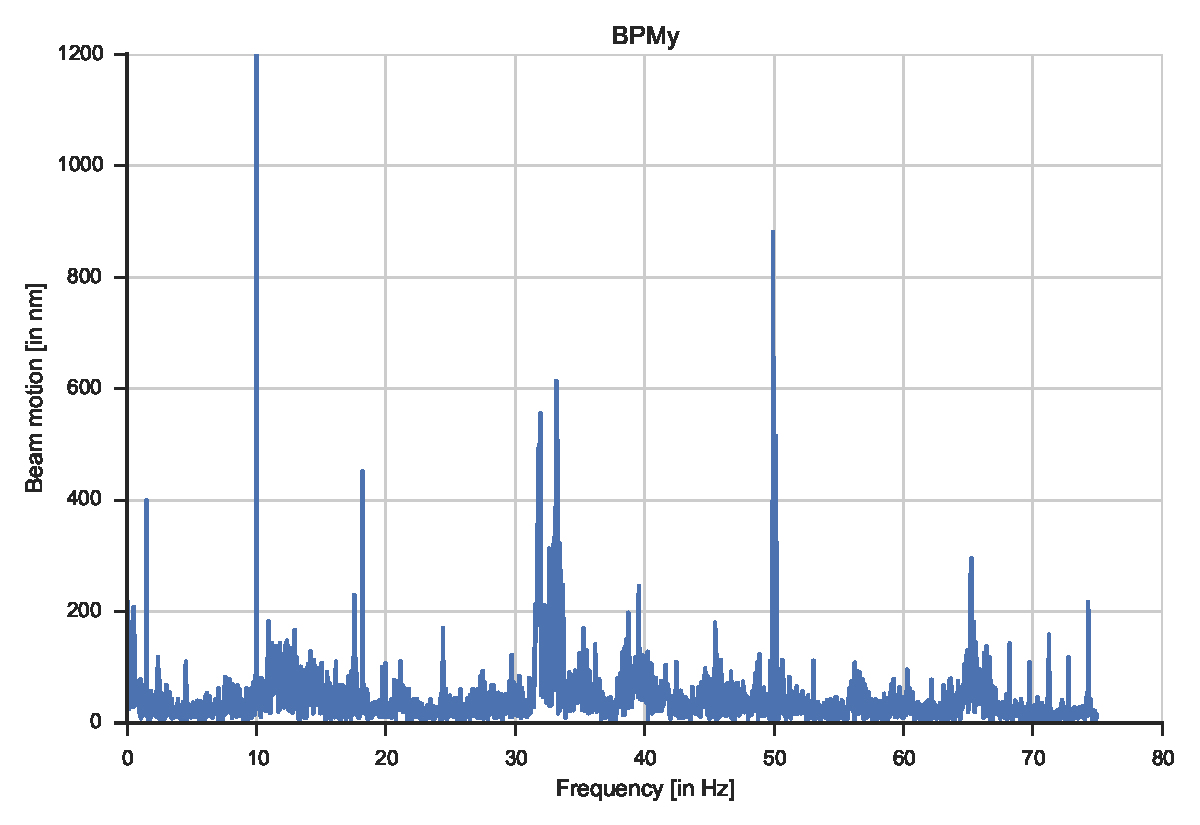
\includegraphics[width=\linewidth]{img/fft_no_corr}
        \caption{No correction}
    \end{subfigure}
    
    \begin{subfigure}[b]{0.8\textwidth}
        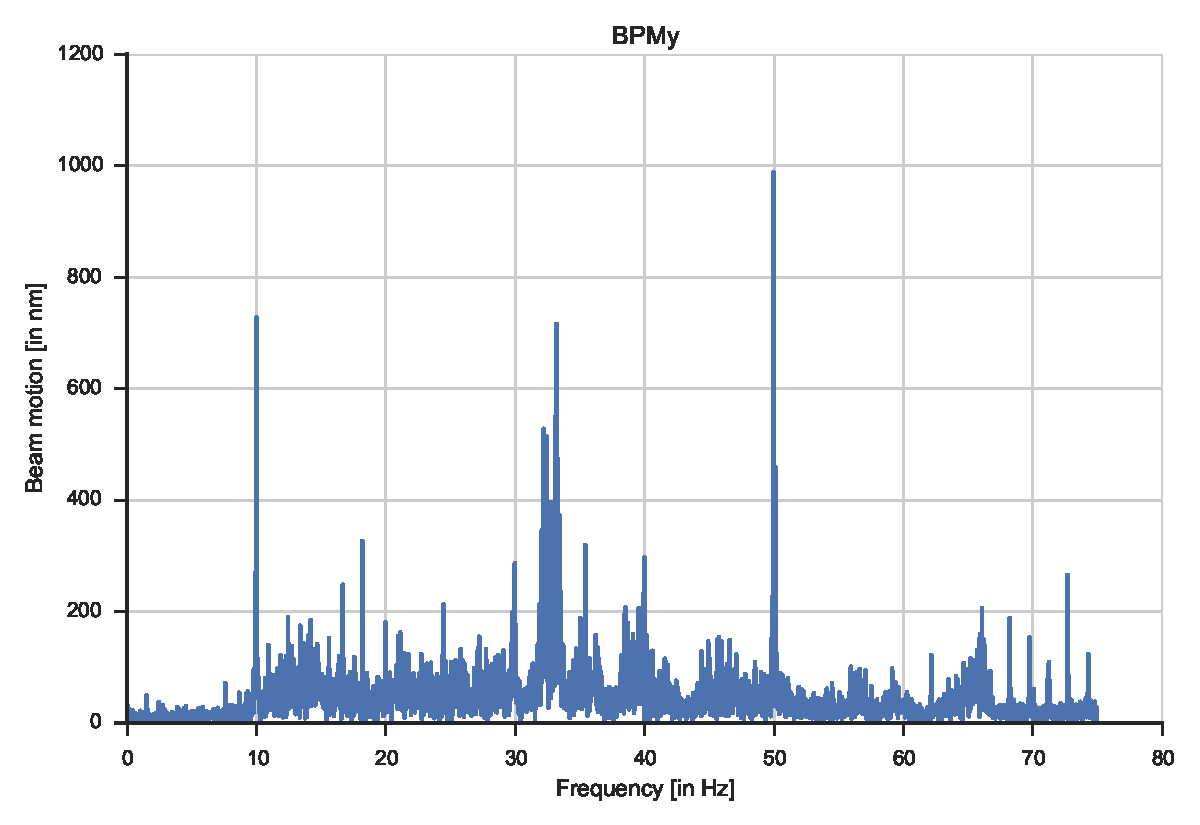
\includegraphics[width=\linewidth]{img/fft_fofb}
        \caption{FOFB correction}
    \end{subfigure}
    \caption{\label{fig:compare_fofb}Orbit motion spectrum: with and without FOFB (vertical)}
\end{figure}

\section{Improvement of the correction for harmonic perturbations}
\label{sec:dyn_corr}
The correction presented until now only provides a correction for the continuous component. It can be seen in \cref{fig:compare_fofb}, that if the correction drastically reduces the perturbations in the lower frequencies (below \SI{10}{\hertz}), frequencies still have high components. This section will provide a method to correct harmonic perturbations.

\subsection{General method}

A simple extension of the previous method is to analyze a given harmonic of the orbit, and consider the Fourier coefficient of each monitor as the complex amplitude of the harmonic orbit of interest
\begin{equation}
	\label{eq:orbit_extract}
	\forall f \in \mathbb{R}, \qquad X_f = \frac{2}{T} \int_0^T x(t) e^{-j 2 \pi f t} dt
\end{equation}
or, in the digital domain,
\begin{equation}
\forall f \in \left[0, \frac{Fs}{2}\right], \qquad X_f = \frac{2}{N} \sum\limits_{k=0}^{N-1} x(k) e^{-j 2 \pi f \frac{k}{F_s}}
\end{equation}
where $F_s$ is the sampling frequency, $f = \frac{1}{T}$ the frequency of interest and $N$ the number of samples.

This method functions because it decomposes the signal in orthogonal functions. With the digitalization, the harmonic function are orthogonal only when the frequency $f$ is a multiple of $\frac{F_s}{N}$. This can be a problem here, as the frequency to analyze might be exactly \SI{10}{\hertz} (see \cref{sec:dyn_corr_ex_10Hz}) and not \SI{9.975}{\hertz} if $N=2000$, $F_s=\SI{150}{\hertz}$. The complex amplitude is therefore used as initial value in a least-square-error algorithm for curve-fitting that will provide a hopefully more precise amplitude if the frequency of interest did met the precedent condition.

This provides an complex differential orbit $\Delta\vec{X}_f$ for the harmonic $f$. From there the corrector values can be calculated with the traditional method
\begin{equation}
\Delta\vec{\Theta}_f = \mat{S}^{1}\, \Delta\vec{X}_f   \in \mathbb{C}^n.
\end{equation}

To apply the correction, an oscillation must finally be generated with the obtained parameters. This is, for the $i$th corrector
\begin{equation}\label{eq:th_dyn_corr}
\forall t \in  \mathbb{R}, \qquad y_i(t) = \left| \Delta\Theta_{f,i} \right| \cdot \cos\left(2 \pi f t - \arg\left(\Delta\Theta_{f,i}\right)\right).
\end{equation}

The main problem with the method as presented here is that the generated signal phase must be synchronized with the time the correction parameters were measured. This is possible only for perturbations for which the source is already known and could be used as reference signal.

\subsection{Example of the 10 Hz perturbation}
\label{sec:dyn_corr_ex_10Hz}
The \SI{10}{\hertz} perturbation has a well known source which is the booster power supply (pre-accelerator). This perturbation has such a great impact on the orbit spectrum and could be used as a validation case.

A coil was used to measure the field generated by a magnet powered by the same source as the booster. It provides a \SI{10}{\hertz} reference which is synchronized with the perturbation.

The orbit and the reference signal were measured during the exact same time. Both were analyzed with the method presented above. Instead of using \cref{eq:th_dyn_corr}, the reference signal was used and its phase and amplitude where changed for each corrector with the help of a finite impulse response (FIR) filter. Because the sampling frequency is \SI{150}{\hertz}, a FIR with $N_\text{taps} = 15$ for the $i$th corrector can be designed as follow
\begin{equation}
	h_i[n] = \frac{2}{N_\text{taps}}\cdot \frac{\left| \Delta\Theta_{f,i} \right|}{\left|A_{10}\right|} \cdot \cos\left(2\pi\cdot \frac{f_{10}}{F_s} n - \left[\arg\left(\Delta\Theta_{f,i}\right) - \phi_{10}\right] \right),\quad n \in 0..N_\text{taps}-1
\end{equation}
where $A_{10}$ and $\phi_{10}$ are respectively the amplitude and the phase of the reference signal, $Fs=\SI{150}{\hertz}$, $f_{10}=\SI{10}{\hertz}$.

This can then be applied to the reference signal $x_{10}$: for the $i$th corrector, the dynamic correction is
\begin{equation}
y[n] = h * x_{10} [n] =  \sum\limits_{k=0}^{14} h[k] \cdot x_{10}[n-k]
\end{equation}

The result of the algorithm is shown in \cref{fig:compare_dyn_corr}. It can be seen that the perturbation is completely removed. Interestingly enough, the FIR filter needed a phase rotation of $-\frac{3}{4}\pi \text{~rad}$ to obtain a good result. It should be noted that the storage ring was filled with low current only.

\begin{figure}
    \centering
    \begin{subfigure}[b]{0.8\textwidth}
        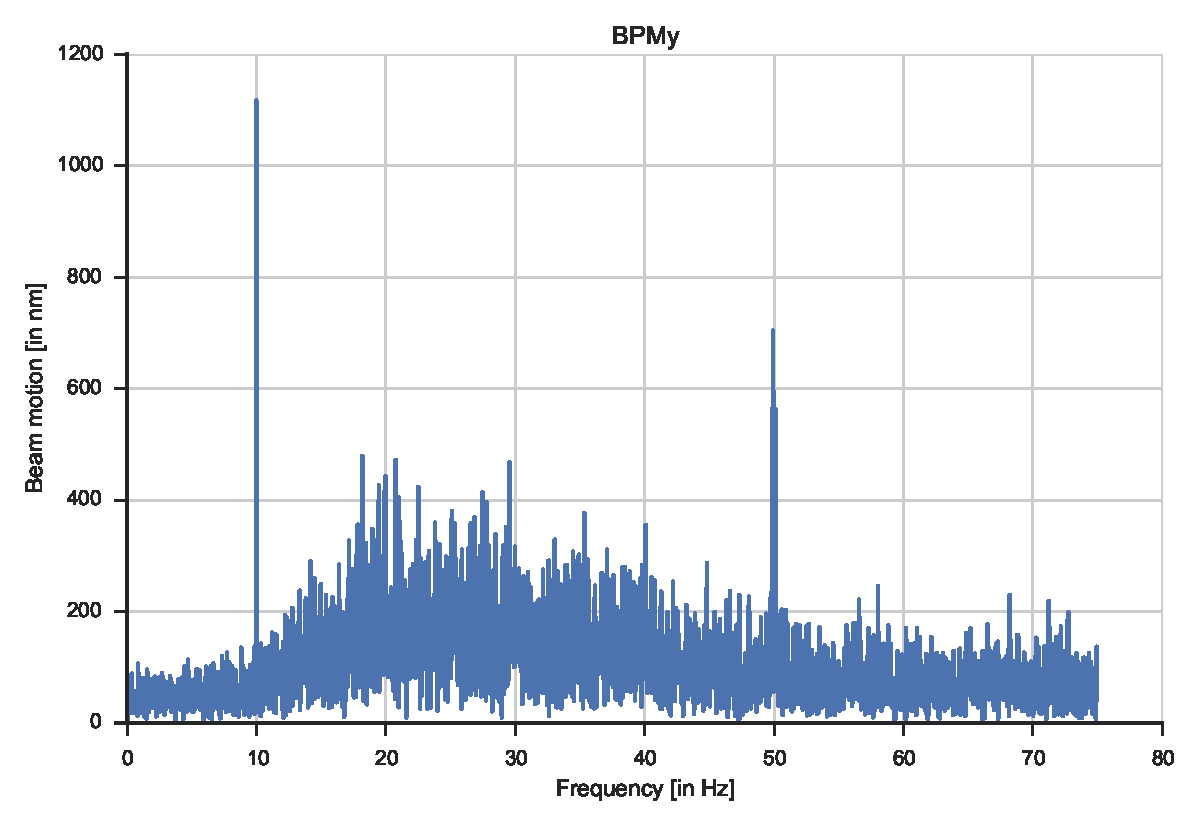
\includegraphics[width=\linewidth]{img/fft_fofb_low}
        \caption{FOFB only}
    \end{subfigure}
%    \hfill
    \begin{subfigure}[b]{0.8\textwidth}
    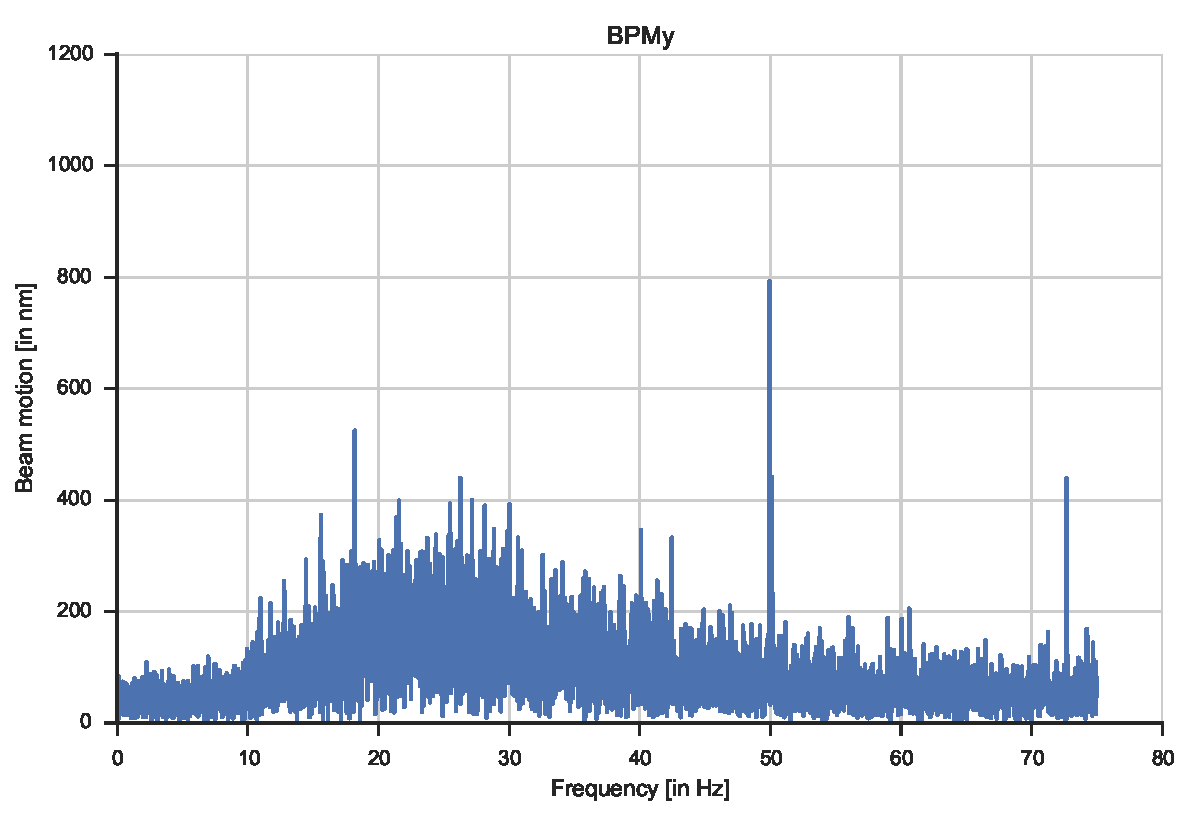
\includegraphics[width=\linewidth]{img/fft_fofb_dyn_low}
    \caption{FOFB + \SI{10}{\hertz} correction}
    \end{subfigure}
    \caption{\label{fig:compare_dyn_corr}Orbit motion spectrum: with and without \SI{10}{\hertz} harmonic correction (vertical)}
\end{figure}


\section{System and correction simulation}
One difficulty in improving the current correction process is that machine time is expensive: tests cannot be done very often. A wrong correction can indeed destabilize the orbit or worse, lose the electrons in the vacuum chamber walls, and thus it cannot be tested when the storage ring is on service or other scientists do experiments or measurements for their own research. However, has presented previously, the process is complex and it must be sure that every actors will play correctly in an improved process. Simulating the whole environment is expected to mitigate this.

\subsection{Theoretical background}
\subsubsection{System}
To model a practical process, a system is used. 

A system is defined as an operator $\mathcal{L}$, changing a set of $q$ inputs $\vec{u}$ in into $p$ outputs $\vec{y}$. Generally, the inputs, outputs and operator can vary with time, position, temperature or any possible variable.

For example if the inputs, outputs and operators are only time dependent:
\begin{equation}
	\vec{y}(t) = \mathcal{L}[\vec{u}(t),t]
\end{equation}

\subsubsection{Linear time invariant system}
A linear time invariant (LTI) system is 
\begin{itemize}
	\item \textbf{time invariant}: the operator $\mathcal{L}$ does not depend of the time, meaning that a given input will always generate the same output: $\mathcal{L}[\vec{u},t]=\mathcal{L}[\vec{u}]$. This is can also being described as
	\begin{equation}
		\vec{y}(t) = \mathcal{L}[\vec{u}(t)] \implies \forall \tau, \quad \vec{y}(t-\tau) = \mathcal{L}[\vec{u}(t-\tau)]
	\end{equation}
	\item \textbf{linear}: 	the operator  $\mathcal{L}$ is linear
	\begin{equation}
		\begin{cases}
			\vec{y}_1(t) = \mathcal{L}[\vec{u}_1(t)] \\
			\vec{y}_2(t) = \mathcal{L}[\vec{u}_2(t)] 
		\end{cases}
		\implies \forall (\alpha, \beta) \in \mathbb{R}^2, \quad
		\alpha \vec{y}_1(t) + \beta \vec{y}_2(t) = \mathcal{L}[\alpha\vec{u}_1(t)+\beta\vec{u}_2(t)]
	\end{equation}
	This linearity property allows analyzing any complicated input as a sum of easier ones that will be superposed. The system complexity can thus be more easily handled.
\end{itemize}

It can be proven that in a LTI system, an harmonic input signal of frequency $f_0$ will produced an harmonic output signal with the same frequency. Only the amplitude and the phase will be different.

\subsubsection{Transfer function}
LTI systems can be described with specific operators called transfer functions.

Let a system with a single input and single output (SISO) be described as 
\begin{equation}
	\label{eq:controlth_diff_eq}
	\sum\limits_{k=0}^M a_k \frac{d^k y}{dt^k}(t) = \sum\limits_{j=0}^N b_j \frac{d^j u}{dt^j}(t).
\end{equation}
Taking its Laplace transform yields
\begin{equation}
\sum\limits_{k=0}^N a_k s^k Y(s) = \sum\limits_{j=0}^M b_j s^j U(s).
\end{equation}
where a $Y(s) = \mathcal{L}\{y(t)\}$ and $U(s) = \mathcal{L}\{u(t)\}$ the Laplace transform of its output and input.

The transfer function is defined as
\begin{equation}
	\label{eq:controlth_tf}
	G(s) = \frac{Y(s)}{U(s)} = \frac{\sum\limits_{j=0}^M b_j s^j}{\sum\limits_{k=0}^N a_k s^k}.
\end{equation}

\begin{itemize}
	\item $N$ is the order of the system (i.e. the order of the pole polynomial) 
	\item $N-M$ is the relative order
	\item A system $G(s)$ is defined as \emph{proper} if $\lim\limits_{\omega \rightarrow \infty} G(j\omega) = D \neq \infty$, which requires $M < N$. It means that it can be physically realized.
\end{itemize}

\subsubsection{State-space description}
If transfer functions are a very useful tool (for example to represent the Bode diagram of a function or easily combine successive systems), computing their outputs is not very practical. Another representation is often used, with the help of a inner variable $x(t)$:
\begin{equation}
\begin{cases}
	\dfrac{d \vec{x}}{dt}(t) &= \mat{A}\,\vec{x}(t) + \mat{B}\, \vec{u}(t) \\
	\vec{y}(t) &= \mat{C}\,\vec{x}(t) + \mat{D} \,\vec{u}(t)
\end{cases}
\quad , \qquad \vec{x}(0) = \vec{x}_0
\end{equation}
where $\mat{A} \in \mathbb{R}^{n \times n}$, $\mat{B} \in \mathbb{R}^{n \times q}$, $\mat{C} \in \mathbb{R}^{p \times n}$ and $\mat{D} \in \mathbb{R}^{p \times q}$ can be defined from the transfer function \cref{eq:controlth_tf} or directly from the differential equation model \cref{eq:controlth_tf}. This will not be described here, as Python and \textsc{Matlab} libraries provide functions to directly calculate the matrices. A more thorough reference can be found in \cite{lect:king-ident}.

This representation is however a continuous representation, that cannot be used directly on a DSP. It must be first be transformed as follow \cite{lect:king-ident}, for a sampling rate $F_s = \frac{1}{T_s}$ 
\begin{equation}
	\mat{\tilde{A}} = e^{\mat{A} T_s}, \quad
	\mat{\tilde{B}} = \int_0^{T_s} e^{\mat{A} (T_s-\tau)} \mat{B} d\tau,\quad
	\mat{\tilde{C}} = \mat{C}, \quad
	\mat{\tilde{D}} = \mat{D}
\end{equation}
and then 
\begin{equation}
\label{eq:controlth_ss}
	\begin{cases}
		\vec{x}[k+1] &= \mat{\tilde{A}}\,\vec{x}[k] + \mat{\tilde{B}}\, \vec{u}[k] \\
		\vec{y}[k] &= \mat{\tilde{C}}\,\vec{x}[k] + \mat{\tilde{D}} \,\vec{u}[k]
	\end{cases}
	\quad , \qquad \vec{x}[0] = \vec{x}_0.
\end{equation}

\Cref{eq:controlth_ss} is mostly used in the simulation algorithm.

\subsubsection{Empirical transfer function estimation}
In some cases, modeling the system with differential equation is either to complex or provides to simplistic results. The system can instead being used as a black box, and it's frequency response measured.

\paragraph{Using Fourier transform}
The Laplace transform evaluated in $s=j\omega$ results in the Fourier transform. Therefore, as shown in \cref{eq:controlth_tf}, using an input with enough frequency content should allow getting a good estimation of the transfer function:
\begin{equation}
	\tilde{G}(j\omega) = \frac{Y(j\omega)}{U(j\omega)}.
\end{equation}
However this naive method is not really used in practice as the measurement noises and artifacts in the output would have strong impact on the estimation.

\paragraph{Spectral density}
A better method is to use the spectral density and the cross-spectral density.

In the time domain, the output can be written as a function of the input by using a impulse response $g(t) = \mathcal{L}^{-1}\{G(s)\}$
\begin{equation}
	y(t) = g * u\,(t) =  \int_0^{+\infty} g(\tau) u(t-\tau)d\tau
\end{equation}

The cross-correlation between the input and the output is given by
\begin{align}
R_{uy}(\tau) &= E \left\{ u(t) y(t+\tau)\right\} \nonumber\\
			 &= E \left\{ u(t) \int_0^{+\infty} g(v) u(t+\tau-v)dv\right\} \nonumber\\
			 &= ... \nonumber \\ 
			 &= \int_0^{+\infty} g(v) R_{uu}(\tau-v) dv \nonumber\\
			 &= g * R_{uu} \, (\tau)
\end{align}
where $R_{uu}$ is the autocorrelation of the input. Transforming this equation to the frequency domain yields
\begin{equation}
	S_{uy}(j\omega) = G(j\omega)\cdot S_{uu}(j\omega)   \iff 	G(j\omega) = \frac{S_{uy}(j\omega) }{ S_{uu}(j\omega)}
\end{equation}
where $S_{uy}$ is the cross-spectral density and $S_{uu}$ the spectral density of the input.

This provides better results in practice because only the relevant information of the signal is used: the transfer function estimation is less dependent of the measurement noise and other possible artifacts.

\paragraph{Correct input}
It is important to choose a good input signal. It must contain enough harmonic components to provide an estimation of the full spectrum. Literature often propose a pink noise or a sine-sweep.

A pink noise is a signal which power spectrum is decreasing like $1/\omega$. The spectrum is thus fully represented, with high frequencies having less impact and therefore being less likely to harm the system. In a system like the storage ring, using a noise as input is however not a good idea. 

A sine sweep is a sine which frequency increases with the time, so that every frequencies are represented. A linear increase can be obtained by setting
\begin{equation}
	f(t) = 2 f_\text{min} \cdot t + \frac{f_\text{max}-f_\text{min}}{2 \cdot t_\text{max}} t^2
\end{equation}
The input is then
\begin{equation}
	u(t) = A \sin(2\pi f(t))
\end{equation}



\subsection{System identification}
The first step in the model is to represent the storage ring. This could be done analytically, by writing the magnet equations and deriving the full differential equations that bind the correction to orbit displacement. However, it would take a full master thesis to realize a good model, as there are very different types of components all around the orbit, with some non-linear, some coupled and complex behaviors.

Instead a system identification is conducted. The system is the storage ring, with the differential orbit as the output, and correction magnet amplitude as input. It is assumed that the system can be modeled as a first approximation as a SISO system, generalized as a MIMO one by pre-multiplying it by the response matrix (which is a mere gain):
\begin{equation}
	\Delta \vec{X}(t) = \mat{S}\cdot \left[ g * \Delta\vec{\theta} \, (t) \right]
\end{equation}

A sine sweep was designed to cover from $f_\text{min} = 0$ to $f_\text{max} = F_s/2 = \SI{75}{\hertz}$ and used as the corrector magnets input (one by one).

By using the (cross-)spectral density of the input and output signal, an experimental estimation of the transfer function is provided. The estimation is then fitted with a \textsc{Matlab} routine implementing the Fast Relaxed Vector Fitting \cite{art:vfit3-1, art:vfit3-2, art:vfit3-3, web:vfit3} and provides the continuous time state-space matrices $\mat{A}$, $\mat{B}$, $\mat{C}$ and $\mat{D}$. The result is shown \cref{fig:ctl_vfit3}.

\begin{figure}
	\begin{subfigure}[t]{0.5\linewidth}
		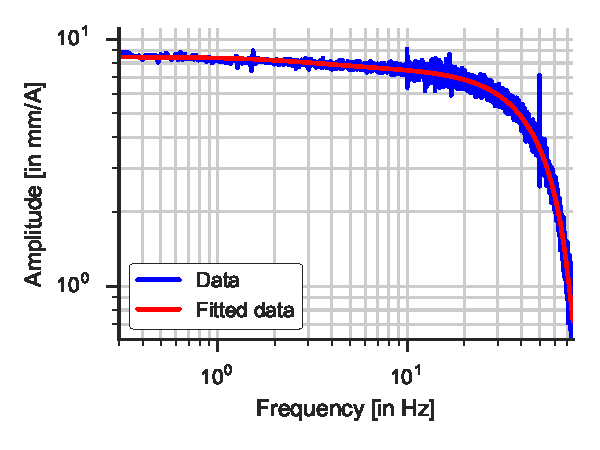
\includegraphics[width=1\linewidth]{img/ctl_id_amplitude}
		\caption{Amplitude}
	\end{subfigure}
	\hfill
	\begin{subfigure}[t]{0.5\linewidth}
		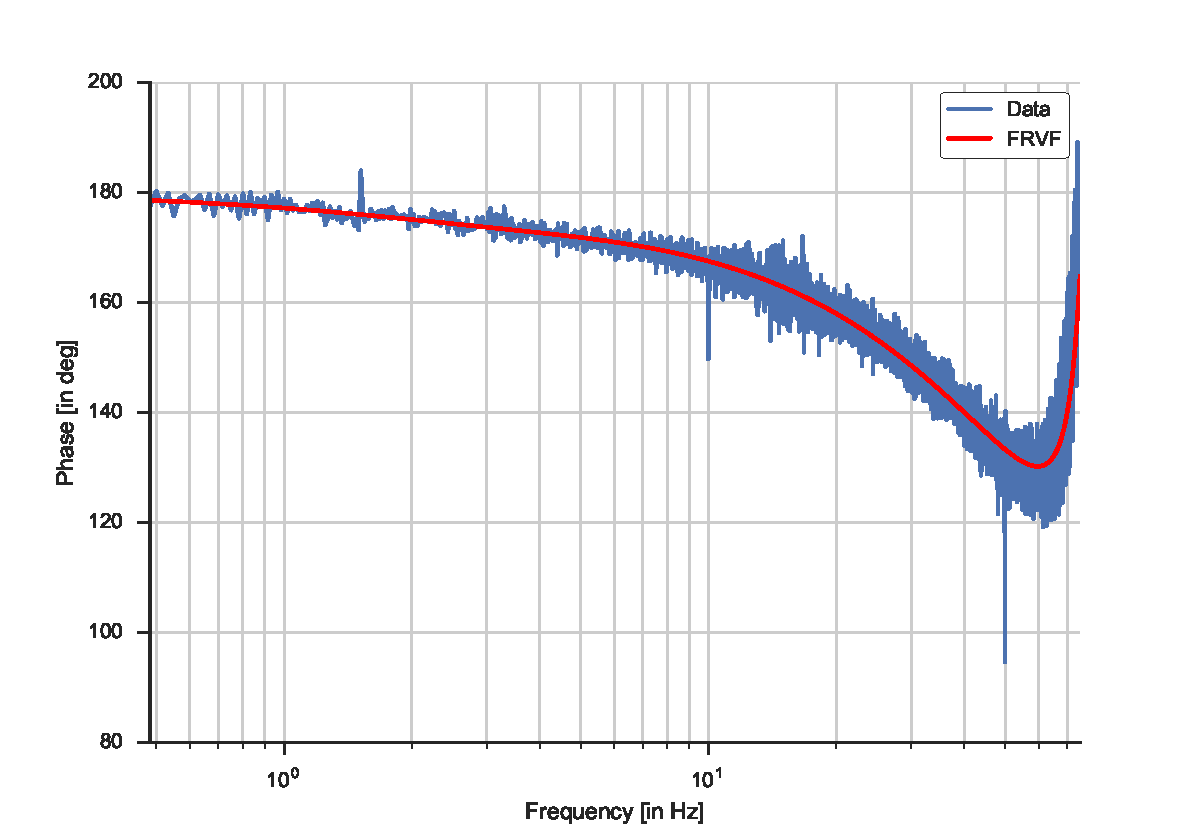
\includegraphics[width=1\linewidth]{img/ctl_id_phase}
		\caption{Phase}
	\end{subfigure}
	\caption{\label{fig:ctl_vfit3}Results of the vector fitting with vfit3}
\end{figure}

It appeared that after converting the system to a transfer function, the numerator was complex. Taking only the real part of each coefficient provided a solution that still fitted the experimental data. In order to obtain a transfer function usable with the response matrix, it was normalized so that its ground gain was 1.

\Cref{fig:ctl_vfit3} shows however only the frequency domain below \SI{75}{\hertz}. In the first simulations, it appeared that the step response presented a large spike which was hardly physically possible (see \cref{fig:ctl_id_spike}). To correct this, the numerator highest degree coefficient was set to 0, which led to the result given in \cref{fig:ctl_id_nospike}. 

\begin{figure}
	\begin{subfigure}[t]{0.5\linewidth}
		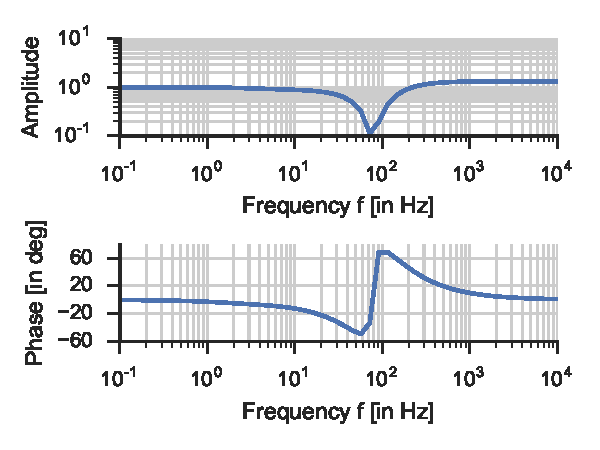
\includegraphics[width=1\linewidth]{img/ctl_id_3z}
		\caption{Frequency response}
	\end{subfigure}
	\hfill
	\begin{subfigure}[t]{0.5\linewidth}
		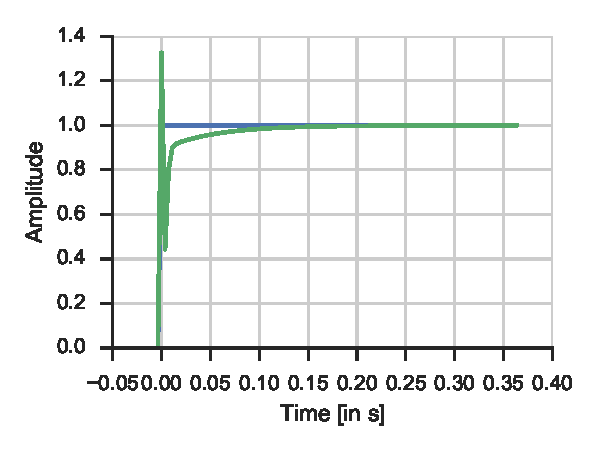
\includegraphics[width=1\linewidth]{img/ctl_id_3z_step}
		\caption{Step response}
	\end{subfigure}
	\caption{\label{fig:ctl_id_spike}Normalized transfer function}
\end{figure}

\begin{figure}
	\begin{subfigure}[t]{0.5\linewidth}
		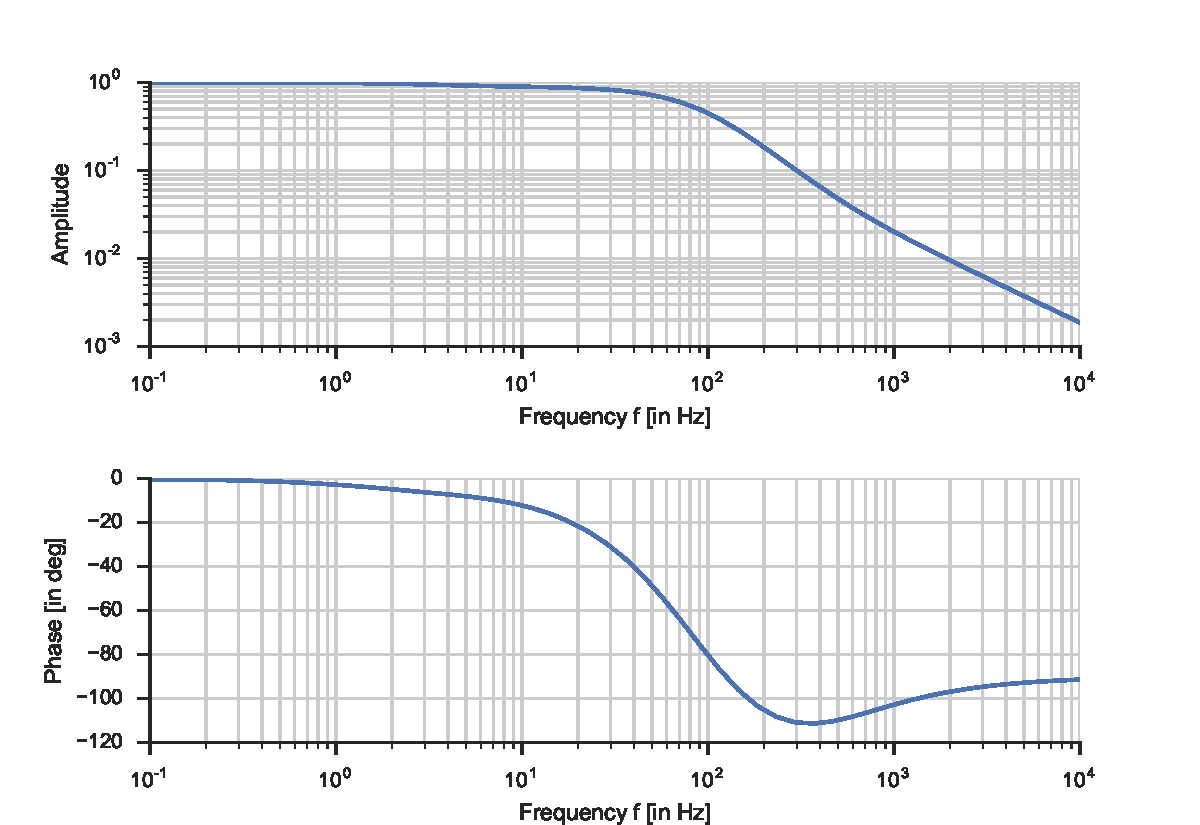
\includegraphics[width=1\linewidth]{img/ctl_id_2z}
		\caption{Frequency response}
	\end{subfigure}
	\hfill
	\begin{subfigure}[t]{0.5\linewidth}
		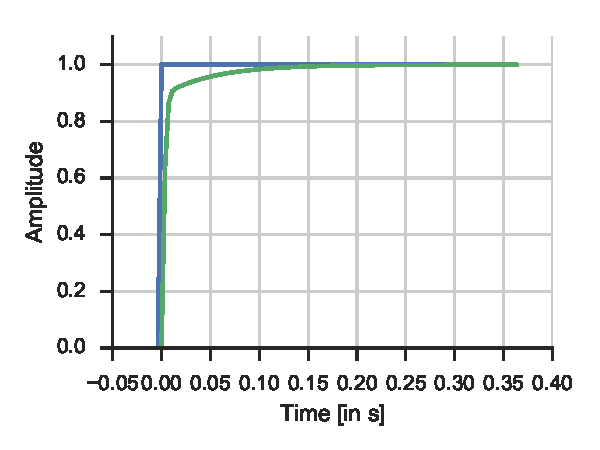
\includegraphics[width=1\linewidth]{img/ctl_id_2z_step}
		\caption{Step response}
	\end{subfigure}
	\caption{\label{fig:ctl_id_nospike}Normalized, zeros-corrected transfer function}
\end{figure}

Finally it the transfer function estimation is 
\begin{equation}
G(s) = \frac{117.322203 \,s^2 + 319144.577 \,s + 6801819.36}
{s^3 + 1171.05630 \,s^2 + 375569.975 \,s +	6801819.36}
\end{equation}

The frequency response given in \cref{fig:ctl_id_nospike} corresponds to what was expected: an amplitude that decreases with frequencies, without amplification domain. To be sure that it corresponds to reality, a simulation of the current situation was conducted.

\subsection{Simulation model}
\label{sec:correction_simulation}

In order to represent at best the environment, the simulation needs to take in account computation delays and that the correction happens at a given sampled time \SI{150}{\hertz}) whereas other systems perform in continuous time. To achieve that, the simulation is played step by step, at \SI{150}{\hertz} for the correction process and \SI{1.5}{\kilo\hertz} for the continuous time.

\Cref{fig:model_simul} represents the block diagram of the environment, $\text{H}_\text{ring}$ being the identified transfer function of storage ring, and the low pass filter representing the averaging of orbit values in the BPM recording. A initial correction $\vec{\theta}_0$, which is normally provided by a punctual correction process (the slow orbit feedback or SOFB), is needed to ensure the stability of the orbit.

\begin{sidewaysfigure}
    \centering
    \begin{tikzpicture}[auto, node distance=1,>=latex']
%    \draw[help lines, yellow] (-1,-4)grid(15,3);
    \draw [dashed, black] (-.5, 1.7) -- (10.1, 1.7) -- (10.1, -3.5) -- (-.5, -3.5) -- cycle;
    \draw [black](2.8, -3.7) node [above right=0 0.2] {\small mBox --- $F_s=\SI{150}{\hertz}$};

    % We start by placing the blocks
    \node [input] (xref) {};
    \node [operator, right=1.5 of xref] (sum) {$+$};
    \node [operator, right=of sum] (xsmat) {$\times$};
    \node [input, above=of xsmat] (smat) {};
    \node [block, right=of xsmat] (corrector) {K};
    \node [operator, right=of corrector] (suminit) {+};
    \node [input, above=of suminit] (initval) {};
    \node [block, right=of suminit] (DAC) {$\uparrow$};
    \node [block, right=of DAC] (delay) {$\begin{matrix}\text{Delay T}\\\text{\footnotesize Computation}\end{matrix}$};
    \node [operator, right=of delay] (sumperturb) {$+$};
    \node [input, above=of sumperturb] (perturb) {};
    \node [block, right=of sumperturb] (Hring) {$\text{H}_\text{ring}$};
    \node [block, below=of delay] (lowpass) {Low pass};
    \node [block, below=of DAC] (ADC) {$\downarrow$ \SI{150}{\hertz}};
    \coordinate [right= of Hring] (connectout) {};
    \node [input, right= of connectout] (out) {};
    
    % Once the nodes are placed, connecting them is easy.
    \draw [->] (xref)     	-- node [pos=0.2] {$\vec{X}_\text{ref}$} (sum);
    \draw [->] (sum)      	-- node {$\Delta\vec{X}$}    	(xsmat);
    \draw [->] (smat)      	-- node {$\mat{S}*$}    	    (xsmat);
    \draw [->] (xsmat)  	-- node {}                   	(corrector);
    \draw [->] (corrector) 	-- node {$\Delta\vec{\Theta}$} 	(suminit);
    \draw [->] (initval) 	-- node {$\vec{\Theta}_0$}      (suminit);
    \draw [->] (suminit)  	-- node {$\vec{\Theta}$}        (DAC);
    \draw [->] (DAC)      	-- node {}                   	(delay);
    \draw [->] (delay)    	-- node {$\theta(t)$}         	(sumperturb);
    \draw [->] (perturb)  	-- node {$d(t)$}               	(sumperturb);
    \draw [->] (sumperturb) -- node {}                		(Hring);
    \draw [-]  (Hring)    	-- node {}                 		(connectout);
    \draw [->] (connectout) -- node {$x(t)$}          		(out);
    \draw [->] (connectout) |- node {}                 		(lowpass);
    \draw [->] (lowpass)    -- node {}                 		(ADC);
	\draw [->] (ADC)     	-| node[pos=0.5] {$\vec{X}$}
                               node [pos=0.90, left]{$-$}	(sum.south);
    \end{tikzpicture}
    \caption{\label{fig:model_simul}The full model, K being the corrector to define}
\end{sidewaysfigure}

\subsection{Simulation results}
Several scenari were designed to validate the simulation, and propose some enhancement to current correction. The delay of the computation is approximated by $\delta t = \SI{3}{\milli\second}$.
 
\subsubsection{Current configuration at BESSY~II}
To represent the current configuration in BESSY~II, the PID corrector presented in \cref{sec:correction_state_of_art} was implemented as a pure integrator of amplitude 0.8. The closed-loop system frequency response would be as given in \cref{fig:ctl_freqresp_pid}. As in the reality, frequencies below \SI{10}{\hertz} are damped, and are slightly amplified above. Applying the simulation step by step with a plausible perturbation leads to the result presented in \cref{fig:ctl_sim_pid}.

\begin{figure}
    \centering
    \begin{subfigure}{0.49\textwidth}
        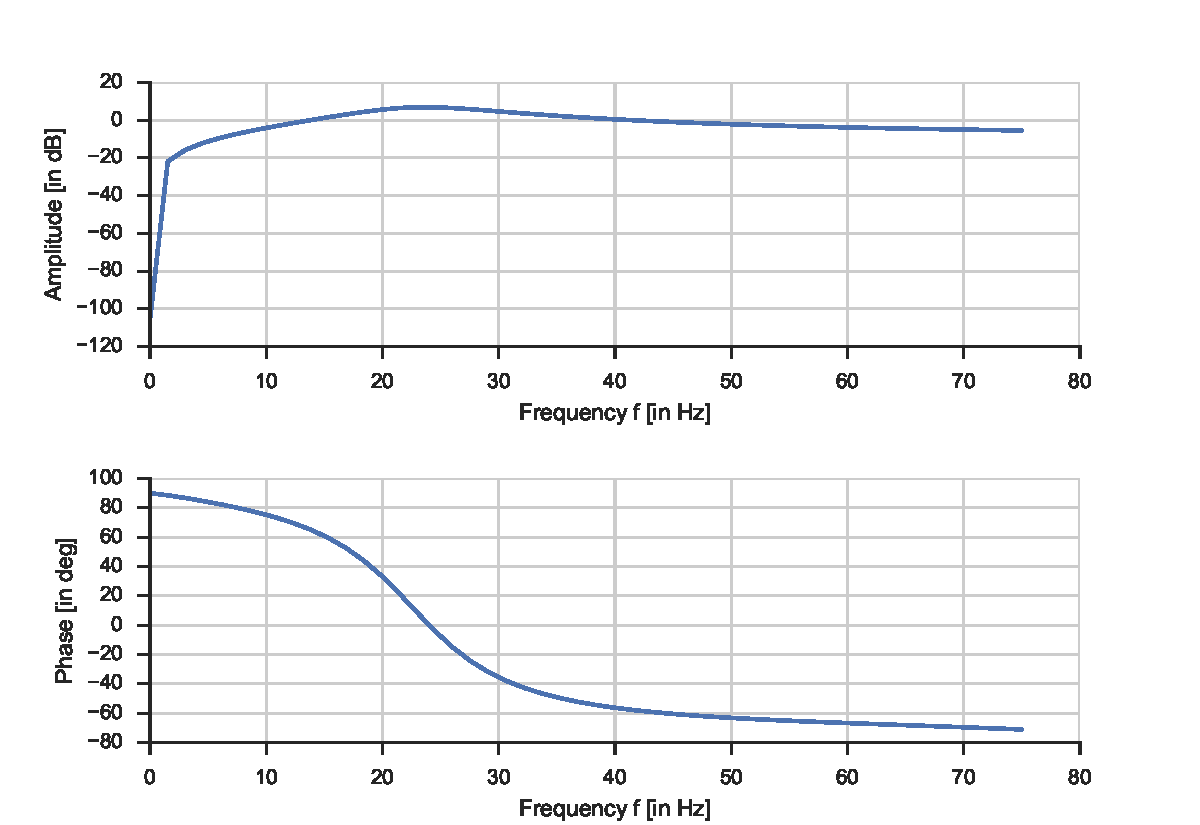
\includegraphics[width=\textwidth]{img/ctl_freqresp_pid}
        \caption{\label{fig:ctl_freqresp_pid} Bode diagram of the closed-loop}
    \end{subfigure}
    \hfill
    \begin{subfigure}{0.49\textwidth}
        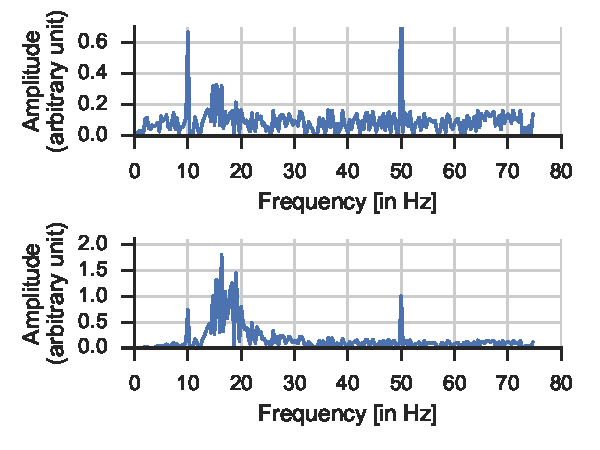
\includegraphics[width=\textwidth]{img/ctl_sim_pid}
        \caption{\label{fig:ctl_sim_pid}Simulation}
        \end{subfigure}    
    \caption{Frequency response for K = PID(0, $0.8\cdot F_s$, 0)}
\end{figure}

The PID can then be slightly enhanced by finding better coefficients, for example with K~=~PID($0.9$, $0.5\cdot F_s$, $0.15/F_s$), which result can be seen in \cref{fig:ctl_freqresp_bestpid,fig:ctl_sim_bestpid}. It can be seen there that more frequencies are slightly damped and that the amplified area is smaller, with less gain, providing better results.

\begin{figure}
    \centering
    \begin{subfigure}{0.49\textwidth}
        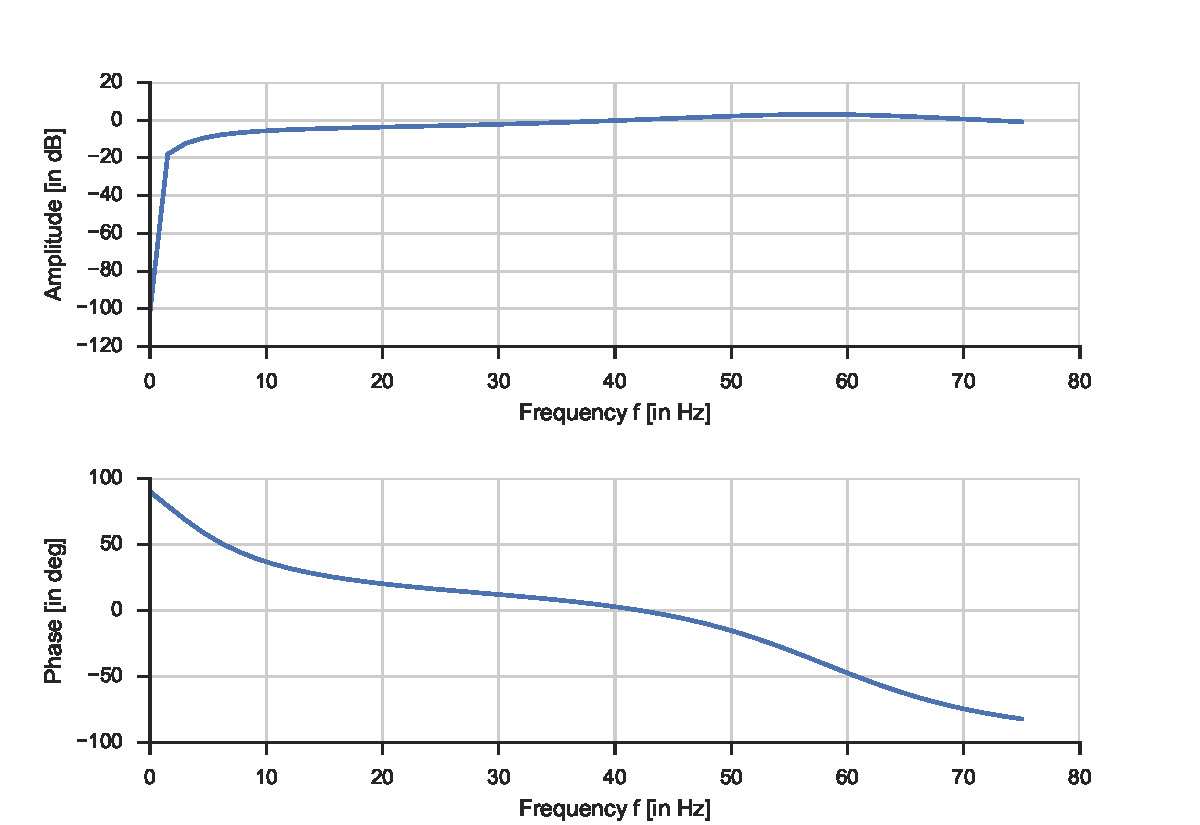
\includegraphics[width=\textwidth]{img/ctl_freqresp_bestpid}
        \caption{\label{fig:ctl_freqresp_bestpid} Bode diagram of the closed-loop}
    \end{subfigure}
    \hfill
    \begin{subfigure}{0.49\textwidth}
        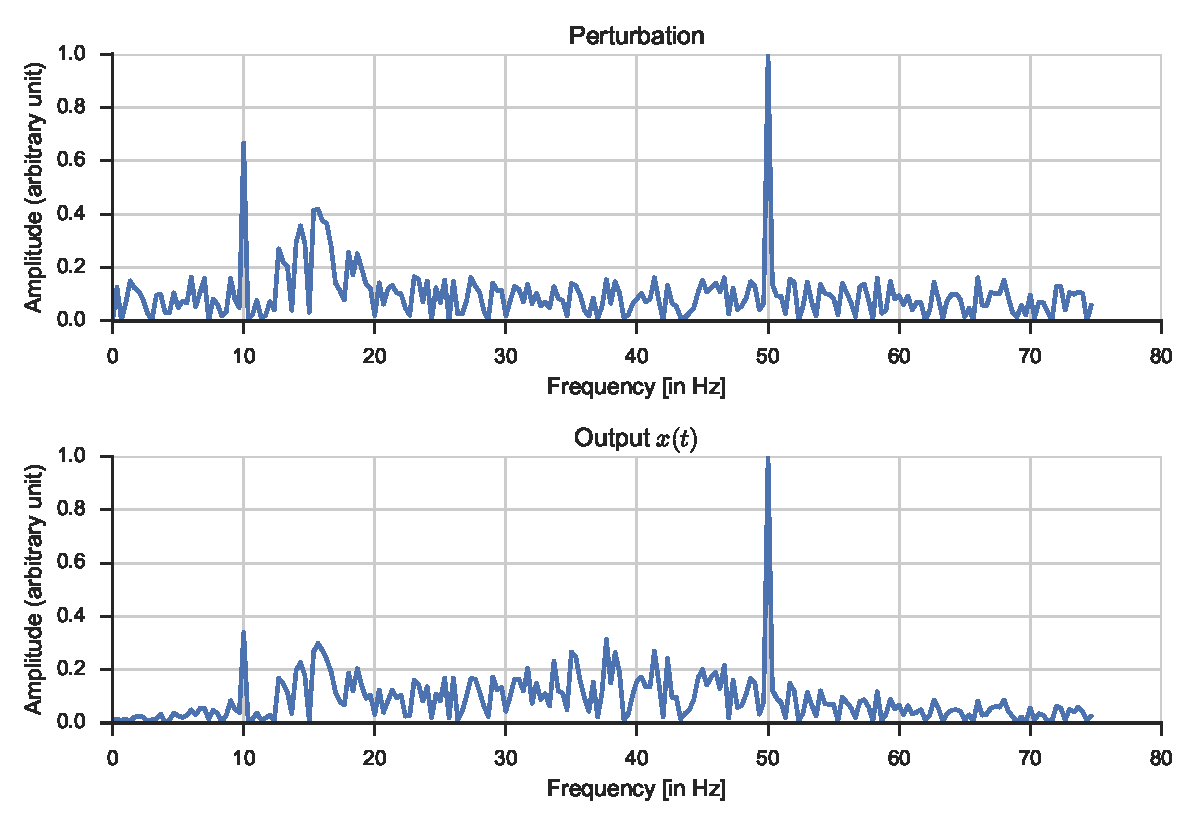
\includegraphics[width=\textwidth]{img/ctl_sim_bestpid}
        \caption{\label{fig:ctl_sim_bestpid}Simulation}
    \end{subfigure}    
    \caption{Frequency response for a better PID}
\end{figure}

\subsubsection{Optimal correction}
Following the design rules defined in \cite{book:Skogestad-2005}, one can synthesize an $\mathcal{H}_\infty$-corrector, which is an optimal corrector obtained by optimizing the closed and opened loop over the $\infty$-norm\footnote{The $\infty$-norm is defined for vectors as $||\vec{x}||_\infty = \max\limits_{i} |x_i|$} with given parameters. The Robust Control Toolbox from \textsc{Matlab} was used for this effect. The \textsc{Matlab} script given below is an adapted copy of what can be found in Skogestad \cite{book:Skogestad-2005}, page 60. The computation delay is modeled with the Padé approximation of first order \cite{book:matrix} provided by \textsc{Matlab} and added to the system, so that the corrector takes this in account.
\begin{Matlab}
% The robust control toolbox is needed.

% Load ring transfert function
[G_num, G_den] = load(G) 

% Create delay
delay = 0.003;
[dnum, dden] = pade(delay, 1);

G = nd2sys(conv(G_num,d_num),conv(G_den,d_den),1);

% Define parameters
fb = 30  % Bandwidth
wb = fb*2*pi;  
M = 1.001;  % Lim sup (high freq.)
Am = 10^-4;  % Lim sup (low freq.)

% Create weights
Wp = nd2sys([1/M wb], [1 wb*Am]);
Wu = 1;

% Define the system
systemnames = 'G Wp Wu';
inputvar = '[r(1) ; u(1)]';
outputvar = '[Wp; Wu; r-G]';
input_to_G = '[u]';
input_to_Wp = '[r-G]';
input_to_Wu = '[u]';
sysoutname = 'P';
cleanupsysic = 'yes';
sysic;

% Compute corrector
nmeas=1; nu=1; gmn=0.5; gmx=20; tol=0.001;
[khinf,ghinf,gopt] = hinfsyn(P,nmeas,nu,gmn,gmx,tol);
\end{Matlab}

This provides a corrector, which frequency response can be seen in \cref{fig:ctl_freqresp_hinf}: very efficient in low frequencies, it has however an amplification area that can be a problem. Correctors with different bandwidth where synthesize. The simulation is given in \cref{fig:ctl_sim_hinf}. The results are strangely enough always less efficient than the proposed PID (in \cref{fig:ctl_freqresp_bestpid}). \todo{$\mathcal{H}_\infty$: Review this part with Maxim}

\begin{figure}
    \centering
    \begin{subfigure}{0.49\textwidth}
        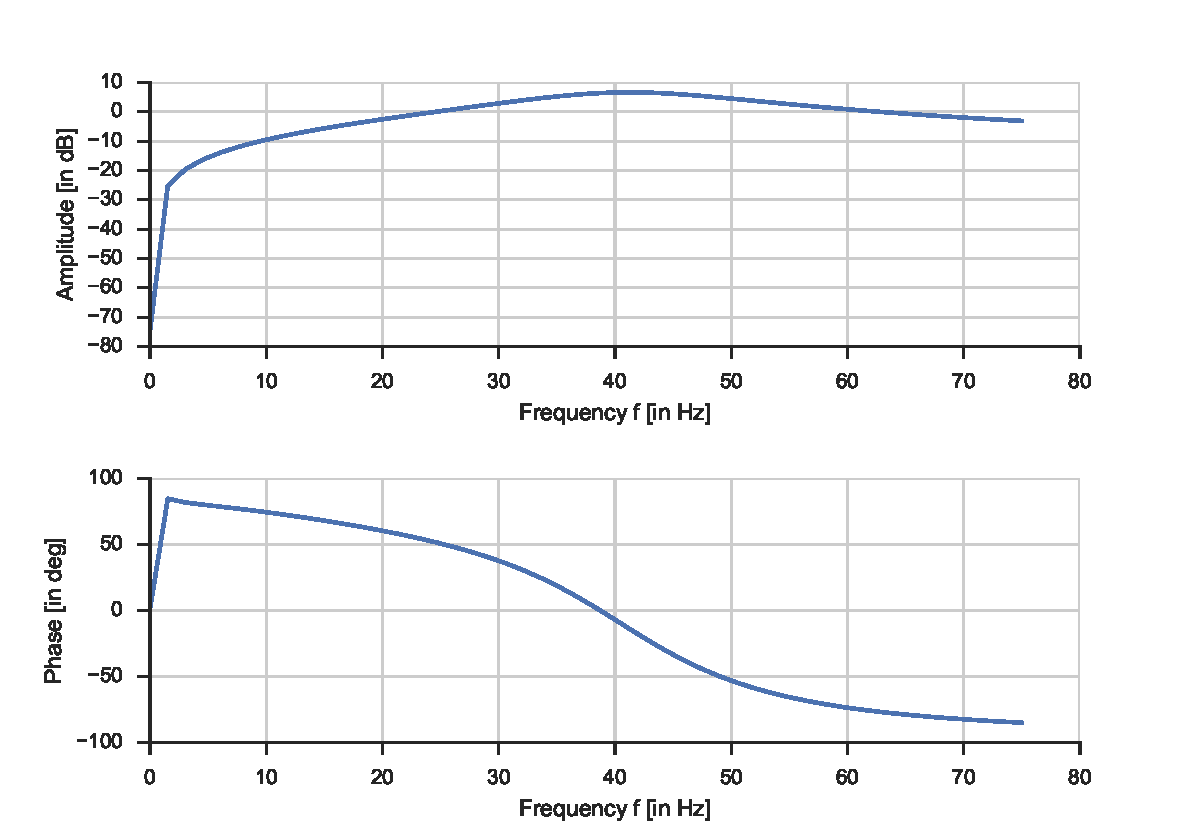
\includegraphics[width=\textwidth]{img/ctl_freqresp_hinf}
        \caption{\label{fig:ctl_freqresp_hinf} Bode diagram of the closed-loop, $f_b$ = \SI{50}{Hz}}
    \end{subfigure}
    \hfill
    \begin{subfigure}{0.49\textwidth}
        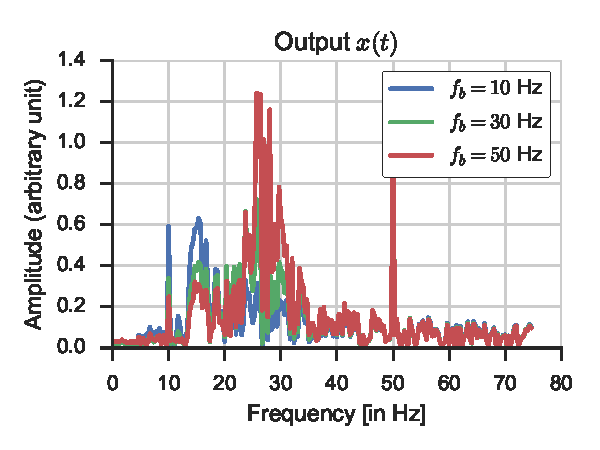
\includegraphics[width=\textwidth]{img/ctl_sim_hinf}
        \caption{\label{fig:ctl_sim_hinf}Simulation (several bandwidths)}
    \end{subfigure}    
    \caption{Frequency response of $\mathcal{H}_\infty$-correctors}
\end{figure}

\section{Summary}
In order to be sure that the electron beam remains focused and stable, a control process is needed. The concerned hardware and software stack at BESSY~II was first studied and the main actor (the mBox) modernized. To the original correction was added a dynamic correction, that can correct static harmonic perturbations and have them almost completely disappear.

In parallel, a simulation environment was built in order to be able to predict the influence of some parameters on the system and to closely study how to correct at best the orbit position. From this was predicted that a more optimized PID corrector is possible, which only needs to be validated experimentally. The optimal correction direction must be considered in more depth and, on a more ambitious perspective, the design of robust MIMO correctors would certainly provide better and more reliable results.
% !TeX encoding = UTF-8
% !TeX spellcheck = en_US
% !TeX root = ../MasterThesis_OlivierChurlaud_2016.tex

\chapter{Localization of orbit perturbations}
\label{sec:localization}

 A correction, as adapted as it can be, will never be perfect. Instead of dealing with the effects of the perturbation, its sources can first be investigated. When all possible sources are found and removed or isolated, a correction algorithm can be applied to the remaining perturbations, which will hopefully yield to better results.

 If no source is really obvious (e.g. a non-isolated transformer, the \SI{50}{\hertz} perturbation of the main power), the orbit itself can give some hints to localize it. One local perturbation affects indeed the whole revolution. It results in an oscillation across the orbit which, because of the closed orbit property, will brutally change its angle at the position of the source  brutally changes its angle (see \cref{fig:kick}). This position is termed \textit{kick}.

\begin{figure}[!h]
	\centering
	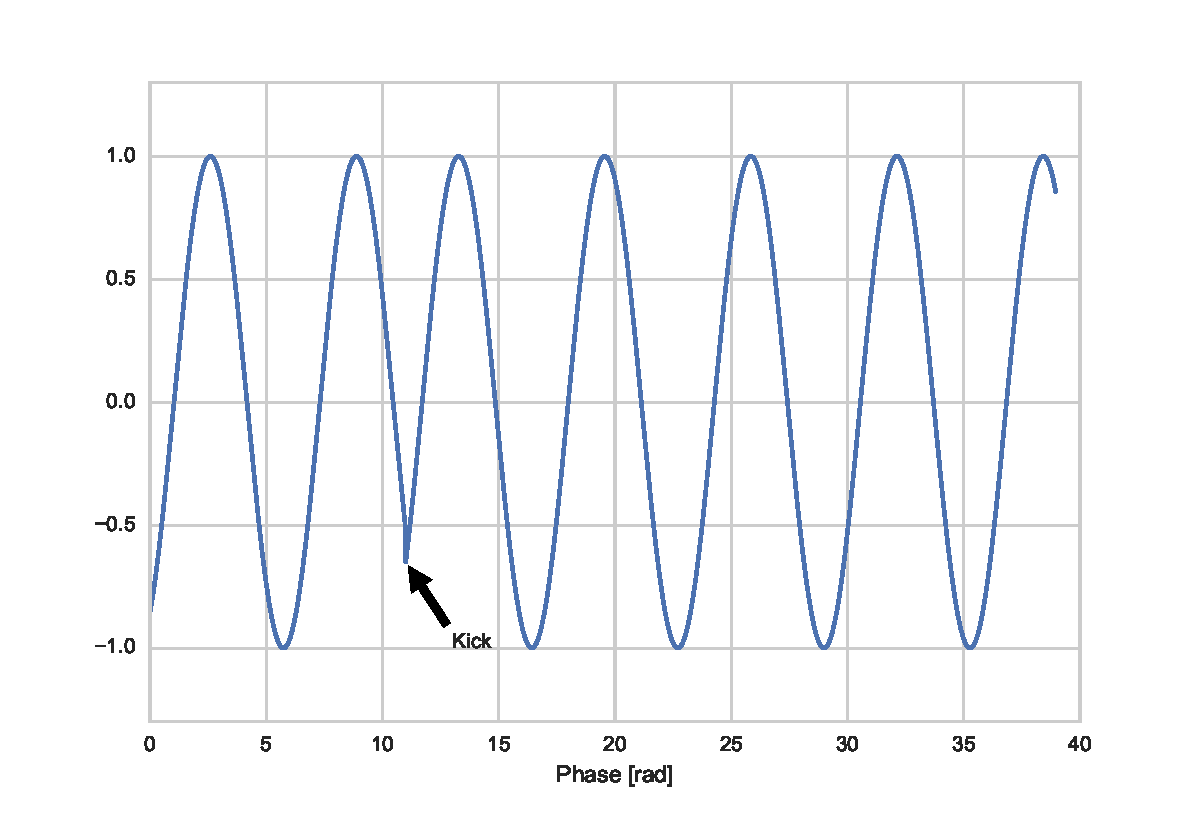
\includegraphics[width=.9\linewidth]{img/kick}
	\caption{\label{fig:kick}Example of kick in the orbit}
\end{figure}

Two types of perturbations will be described in this section:
\begin{itemize}
	\item static perturbations, which can be  for instance a malfunctioning magnet,
	\item harmonic perturbations, i.e. a perturbation at a given frequency, which can be for instance the \SI{50}{Hz} magnetic field of the main power or the \SI{10}{Hz} field due to a bad isolated power supply.
\end{itemize}

\section{Static perturbation}
\label{sec:loc_static}

\subsection{Theoretical setting of the problem}
The problem is described with the betatron phase variable
\begin{equation}
\Psi = \int\limits_{0}^s \frac{d\sigma}{\beta(\sigma)}.
\end{equation}

The spatial variable $s$ is only used to have a connection between the result and the actual ring. The explanation will be led in the horizontal plane (with the $x$ variable), but is also valid in the vertical one ($y$).

Let one kick be at a given phase $\Psi = \hat{\Psi}$. The orbit is modified and oscillates with a constant period of \SI{2 \pi}{\radian}. Because there is \emph{only one} kick and according to the closed orbit condition, the oscillation after the kick will be stable for one revolution. Furthermore, the orbit must be continuous on all points, thus at the kick position too. This is illustrated in \cref{fig:kick}.

Two revolutions are considered, in order to be sure to find one full revolution without kick. Let $\Psi^\mathrm{ext} \in [0, 4 \pi Q]$ be this new phase (\textit{ext} for extended). The phase $\hat\Psi$ where the kick happens is the one so that
\begin{equation}
\exists (b, c) \in \mathbb{R}^2:
\forall \Psi \in [\hat\Psi, \hat\Psi + 2 \pi Q], \quad
x(\Psi) = b \cos(\Psi + c)
\end{equation}
where Q is the tune of the orbit (see \cref{eq:tune}).

This problem has 3 unknowns which should be determined: $\hat\Psi, b, c$.

\subsection{Practical setting}
In order to know the position of the orbit, BPMs are used.

Only $m$ BPMs are distributed around the orbit. The previous variable can thus be described in a vectorial form
\begin{align}
\begin{cases}
\vec{\Psi} = [\Psi_0, \Psi_1, ..., \Psi_{m-1}] \\
\vec{x} = [x_0, x_1, ..., x_{m-1}]
\end{cases} \quad \mathrm{and} \quad
\begin{cases}
\vec{\Psi}^\mathrm{ext} = [\vec{\Psi}, \vec{\Psi}+2\pi Q ]\\
\vec{x}^\mathrm{ext} = [\vec{x}, \vec{x}]
\end{cases}
\end{align}

\subsection{Solving the problem}

The problem is solved in two steps: first the sine that fits at best the orbit is determined, and second the position of the kick verifying the closed orbit condition (or continuity condition) is found.

An algorithm is designed to find a sine over a revolution, beginning at each BPM and keep the one that fits at best:
\begin{align}
\forall~k \in \, &[0,m-1], \nonumber \\
&\begin{cases}
\vec{\Psi}^k = [\vec{\Psi}_\mathrm{ext}(k), \vec{\Psi}_\mathrm{ext}(k+1), \cdots,  \vec{\Psi}_\mathrm{ext}(k+m-1)]\\
\vec{x}^k = [\vec{x}_\mathrm{ext}(k), \vec{x}_\mathrm{ext}(k+1), \cdots,  \vec{x}_\mathrm{ext}(k+m-1)]\\
\tilde{\vec{x}} = \mathtt{fit\_sine}(\vec{x}^k, \vec{\Psi}^k)
\end{cases}
\end{align}

\begin{align}
\forall~k \in \, &[0,m-1], \nonumber \\
&\begin{cases}
\vec{\Psi}^k = [\Psi^\mathrm{ext}_{k}, \Psi^\mathrm{ext}_{k+1}, \cdots,  \Psi^\mathrm{ext}_{k+m-1}]\\
\vec{x}^k = [x^\mathrm{ext}_{k}, x^\mathrm{ext}_{k+1}, \cdots,  x^\mathrm{ext}_{k+m-1}]\\
\tilde{\vec{x}} = \mathtt{fit\_sine}(\vec{x}^k, \vec{\Psi}^k)
\end{cases}
\end{align}

It is then defined
\begin{equation}
k_0 = \underset{k \in [0, m-1]}{\textrm{argmin}}\{||\tilde{\vec{x}}-\vec{x}^k||_2\}
\end{equation}

If there where no noise in the signal, and if the number $m$ of BPMs was infinite, then the kick would be exactly at $\Psi_{k_0}$. However in the real case (with noise), it can only be said that the kick is around $\Psi_{k_0}$, and the closest sine is $\tilde{x}(\Psi) = b \sin(\Psi + c)$.

To find the exact position of the kick, the property of closed orbit is used: the orbit must be continuous also at the kick phase, which means that $\hat{\Psi}$ is the solution of
\begin{align}
b \cos(\Psi + c) &= b\cos(\Psi+c+2 \pi Q),\\
& \mathrm{with}~ \Psi \in [\Psi_{k_0}-A, \Psi_{k_0}+A] , A>0 \nonumber
\end{align}
\begin{align}
&\begin{cases}
\Psi + c &\equiv \Psi + c + 2 \pi Q \pmod{2 \pi} \\
\Psi + c &\equiv - (\Psi + c + 2 \pi Q) \pmod{2 \pi}
\end{cases} \nonumber\\
\iff &\begin{cases}
2 \pi Q &\equiv 0\pmod \pi \qquad\qquad\textit{(Never true)}\\
\Psi &\equiv -c - \pi Q  \pmod \pi
\end{cases} \nonumber
\end{align}

The only possible solutions have the form
\begin{equation}
 \Psi \equiv - c - \pi Q \pmod \pi.
\end{equation}
As the kick is the closest solution to $\Psi_{k_0}$, a constant $K$ is searched so that
\begin{gather}
 -c - \pi Q + K \pi  \leq \Psi_{k_0} \leq -c -\pi Q + (K+1) \pi \nonumber \\
\iff \frac{\Psi_{k_0} + c}{\pi} + Q \leq K \leq \frac{\Psi_{k_0} + c}{\pi} + Q + 1 \nonumber \\
\iff K = \left\lfloor  \frac{\Psi_{k_0}+c}{\pi} + Q \right\rfloor 
\end{gather}
and the two remaining possible values are
\begin{equation}
\left\lbrace - c - \pi Q+ K \pi , \quad - c - \pi Q + (K+1) \pi\right\rbrace
\end{equation}
the kick being chosen as the closest one from $\Psi_{k_0}$.

\subsection{Finding the good sinusoidal}
Several methods are possible to find the best matching sine, for example by using:
\begin{itemize}
	\item a pseudo-inversion
	\item a scalar-product with a sine (resp. a cosine)
\end{itemize}

\paragraph{Pseudo-inversion}
The problem can be set as a linear equation problem as follow.
\begin{align}
&\forall k \in [0,m-1], \tilde{x}(\Psi_k) = a_1 \cos(\Psi_k) + a_2 \sin(\Psi_k) + a \nonumber \\
%
\implies &
\begin{pmatrix}
1 & \cos(\Psi_0) & \sin(\Psi_0) \\
1 & \cos(\Psi_1) & \sin(\Psi_1) \\
\vdots & \vdots & \vdots \\
1 & \cos(\Psi_{m-1}) & \sin(\Psi_{m-1}) \\
\end{pmatrix}
\begin{pmatrix}
a \\ a_1 \\ a_2
\end{pmatrix}
=
\begin{pmatrix}
x_0 \\ x_2 \\ \vdots \\ x_{m-1}
\end{pmatrix} \nonumber
\\
%
\implies &
\begin{pmatrix}
a \\ a_1 \\ a_2
\end{pmatrix}
=
\mathrm{pseudo\_inv}
\begin{pmatrix}
1 & \cos(\Psi_0) & \sin(\Psi_0) \\
1 & \cos(\Psi_1) & \sin(\Psi_1) \\
\vdots & \vdots & \vdots \\
1 & \cos(\Psi_{m-1}) & \sin(\Psi_{m-1}) \\
\end{pmatrix}
\begin{pmatrix}
x_0 \\ x_2 \\ \vdots \\ x_{m-1}
\end{pmatrix}
\end{align}

The pseudo inverse is calculated in \texttt{Matlab} with
\begin{verbatim}
        a = M\x
\end{verbatim}
and in \texttt{Python} with the least-squares method
\begin{verbatim}
        a = numpy.linalg.lstsq(M, x).
\end{verbatim}

\paragraph{Projection on cosine/sine planes}
Since the orbit is expected to be written as
\begin{equation*}
x(\Psi) = a+ a_1 \cos(\Psi) + a_2 \sin(\Psi)
\end{equation*}
it can also be described as
\begin{equation}
x(\Psi) = \scal{x}{1} + \scal{x}{\cos} \cos(\Psi) + \scal{x}{\sin} \sin(\Psi)
\end{equation}
with $\scal{f}{g}$ being the scalar product for real functions: $\int_T f(t)g(u)dt$.

In the numerical case, the scalar product is approximated by its vectorial counterpart by
\begin{align*}
\scal{\vec{f}}{\vec{g}}: \quad
 &\mathcal{R}^n \times \mathcal{R}^n \longrightarrow \mathcal{R} \\
 & (\vec{f},\vec{g}) \quad\longmapsto \quad \frac{1}{n}\sum\limits_{k=0}^{n-1} f_i g_i
\end{align*}

This however provides less good results, as $\sin(\Psi)$ and $\cos(\Psi)$ are numerically orthogonal only if the frequency is a multiple of the sampling frequency divided by the number of samples ($F_s/N$) which cannot be always verified.

\paragraph{Coefficient format}
By defining $b = \sqrt{a_1^2+a_2^2}$ and $c = -\mathrm{arg}(a_1 + j a_2)$ the previous formulas can be written
\begin{equation*}
\tilde{x}(\Psi) = a + a_1 \cos(\Psi) + a_2 \sin(\Psi) = a + b \sin(\Psi + c).
\end{equation*}


\section{Harmonic perturbations}
Some perturbations can be purely harmonic. The example of the \SI{50}{\hertz} field generated by the main power is an obvious one that cannot be easily isolated. 

As the shown in \cref{fig:compare_fofb}, the correction leaves some spikes in the spectrum, some of which hopefully allowing to be localized\todo{this doesn't sound proper english} and removed or isolated.

Because the storage ring is considered in a first approximation as a linear system, the source of an harmonic perturbation can be localized as an harmonic disturbance with the same frequency. The same very same algorithm can thus be used on a pseudo-orbit extracted from the harmonic of interest. 

The harmonic orbit is calculated the same way as in \cref{sec:dyn_corr}, \cref{eq:orbit_extract}, providing a complex vector $\Delta\vec{X}_f$.

\subsection{Case of a unique perturbation source}
If the perturbation is unique, then it is expected to be writable as $d(t) = A_d\cos(2\pi f t + \phi)$ and, because the phase shift is the same for all BPMs, the orbit time signal for the $i$th BPM as 
\begin{equation}
	x_i(t) = \hat{X}_{f,i} \cos (2\pi f t), \qquad \hat{X}_{f,i} \in \mathbb{R}.
\end{equation}
All complex amplitude must thus exactly describe the same sinusoid of frequency $f$ and phase $\alpha_0$, only the amplitude being different at each BPM.
The complex vector $\Delta\vec{X}_f$ can thus be fully described by their amplitudes.

However, since the signal contains also noise and that the perturbation \emph{might} not be unique, it is rotated until the vector of sine (or imaginary part) is minimal, or zero in a ideal case.
\begin{equation}
\begin{cases}\alpha_0 = \underset{\alpha \in [0, 2\pi[}{\textrm{argmin}}\{\Imag{\Delta\vec{X}_f \cdot e^{-j\alpha}} \} \label{eq:harm_perturb_opt}\\
\vec{\hat{X}}_f = \Real {\Delta\vec{X}_f \cdot e^{-j\alpha_0}}
\end{cases}
\end{equation}

This way only one perturbation is considered: the one which contributes the most to the signal.

The new signal $\vec{\hat{X}}_f$ can be used as an differential orbit signal. The kick position is then calculated it with the method described in the static case, \cref{sec:loc_static}.

\remark To achieve the phase optimization given in \cref{eq:harm_perturb_opt}, the Karhunen–Loève transform (or principal component analysis) can be used~\cite{book:wang_2012}. A description of the algorithm is given in \cref{apx:KLT}. If the results are exactly the same, this allows the problem to be solved within a broader theoretical setting. The goal is not anymore to see the sine part vanish but to deal with the perturbation space in which the distortion is the largest. In theory, dealing with each principal component would allow to find the position of each perturbation source.

\subsection{Case of several perturbation sources}
If there are several perturbation sources, a $\alpha_0$ that let the sine part vanish cannot be found.
\todo[inline]{So what do we do? do it until all localized? or drop the section?}

\section{Experimental results}
\subsection{Artificial static perturbation}
The localization presented above is used on an artificial experiment. All correctors are set to 0, except one which is randomly chosen and given an arbitrary amplitude. The orbit is generated by using the response matrix (see \cref{sec:response_matrix}) and provides the curve presented in green on \cref{fig:loc_orbit} (in blue is the final localization).

\begin{figure}
    \centering
    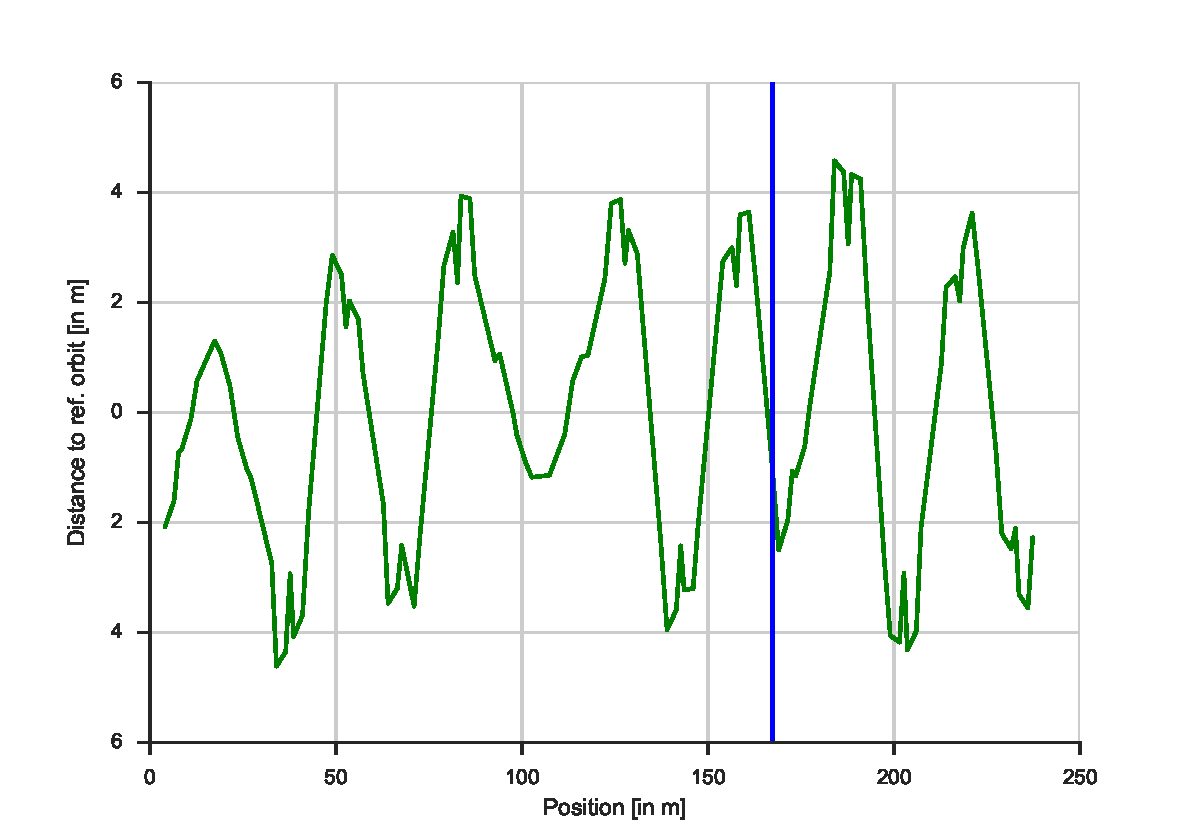
\includegraphics[width=\linewidth]{img/loc_orbit}
    \caption{\label{fig:loc_orbit} Orbit with unique static perturbation}
\end{figure}

The localization algorithm iterations are shown in \cref{fig:loc_errorplots}. The top graph presents in blue the RMS errors between the orbit and a generated sine while setting the kick at each BPM. In green and red are respectively the best fitting amplitudes and phases for each iteration. The convergence is visible and verifies that there are very few risk of being far from the position of the perturbation. However the region where the RMS reaches its smallest value is very flat and thus not very precise.

\begin{figure}
    \centering
    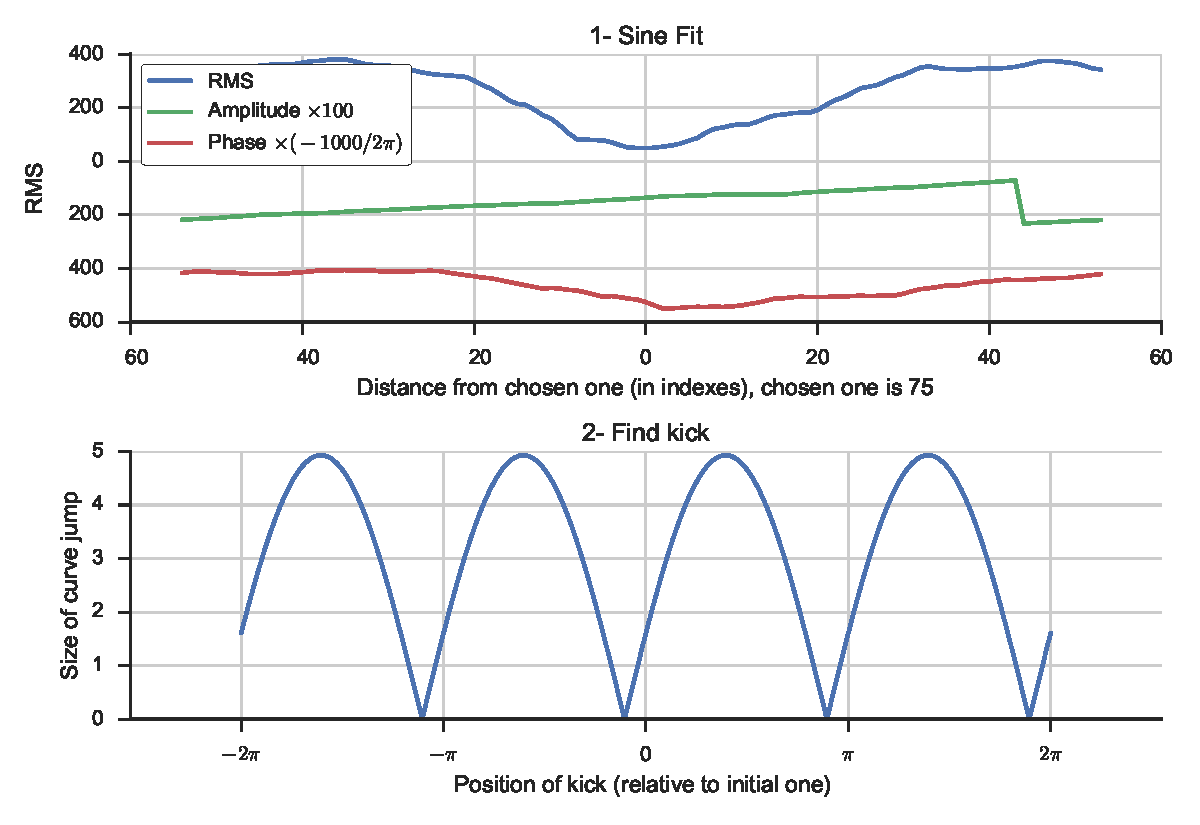
\includegraphics[width=\linewidth]{img/loc_errorplots}
    \caption{\label{fig:loc_errorplots} Error (RMS) and parameters curve of the localization algorithm}
\end{figure}

What is worth remarking is that the amplitude and phase vary quite continually, meaning that choosing the wrong position to set the sinus parameters is not too harmful. This validates the idea of first setting the sinusoid parameters and then find the exact position of the kick.

On the second graph (\cref{fig:loc_errorplots}, below) is represented the jump done by the curve left and right from the BPM chosen to set the sinusoid parameters. In the algorithm, the first minimum of the curve is defined as the kick position.

Finally on \cref{fig:loc_reconstructed_sine} can be seen the orbit and the sinusoid constructed by the algorithm. They are quite overlapping and the closed orbit condition is verified.

\begin{figure}
    \centering
    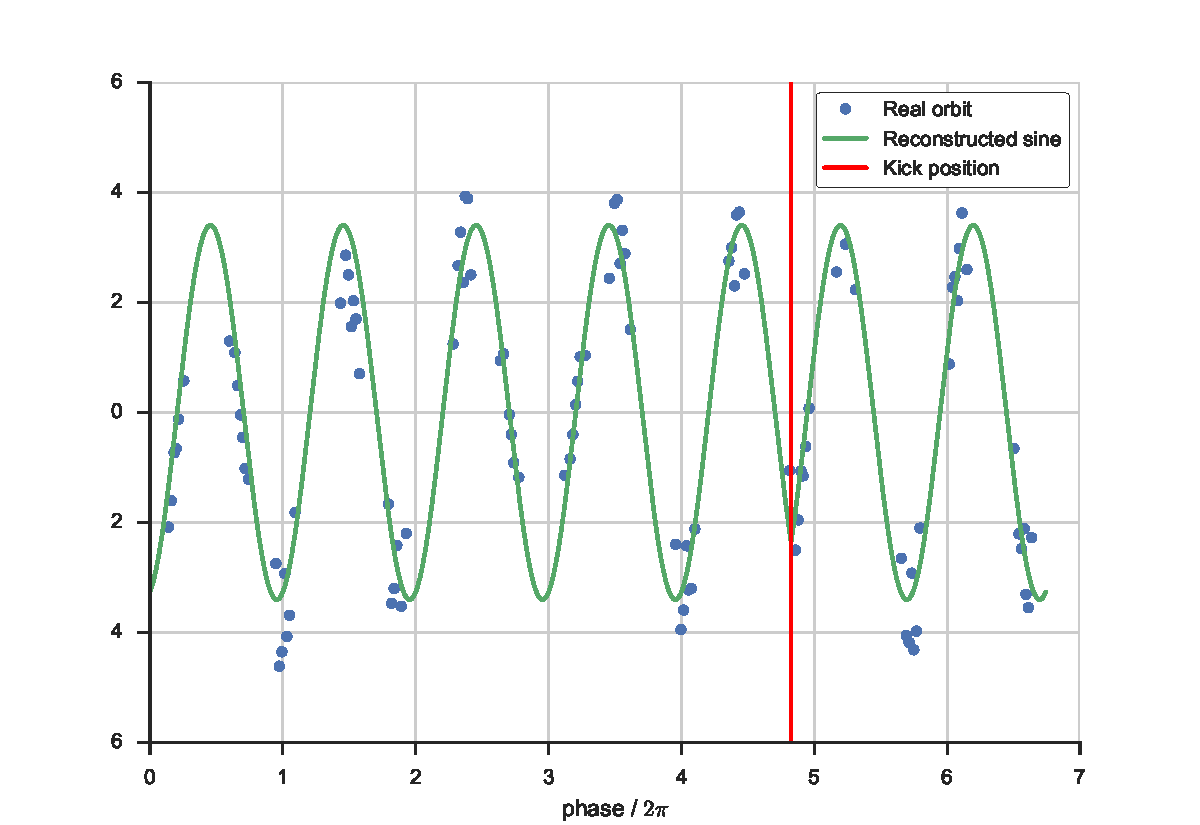
\includegraphics[width=\linewidth]{img/loc_reconstructed_sine}
    \caption{\label{fig:loc_reconstructed_sine} Reconstructed sinusoid and orbit}
\end{figure}

The same artificial experiment was conducted by setting each corrector separately to an arbitrary value and trying to localize it back. \Cref{fig:loc_all_corr} shows the results. It appears that the localization error in such an environment is quite precise in the vertical direction ($d \approx \SI{2}{\meter}$ on a ring of \SI{240}{\meter}), except for the 11th corrector, and a little less in the horizontal direction. However it still reduces a lot the area where to physically search for a source of magnetic perturbation.\todo{Conclusion: This should be studied in the future}

\begin{figure}
    \centering
        \begin{subfigure}[b]{0.6\textwidth}
            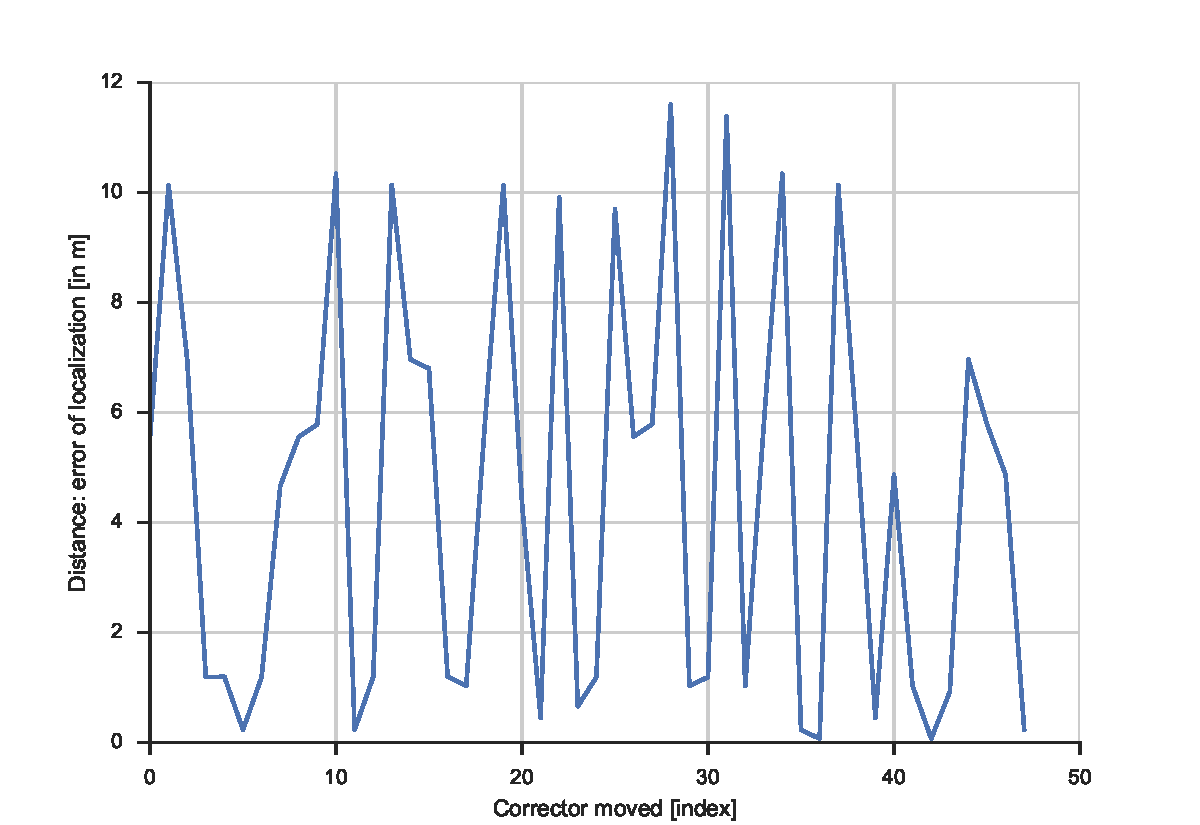
\includegraphics[width=\linewidth]{img/loc_all_x}
            \caption{Horizontal}
        \end{subfigure}
        \begin{subfigure}[b]{0.6\textwidth}
            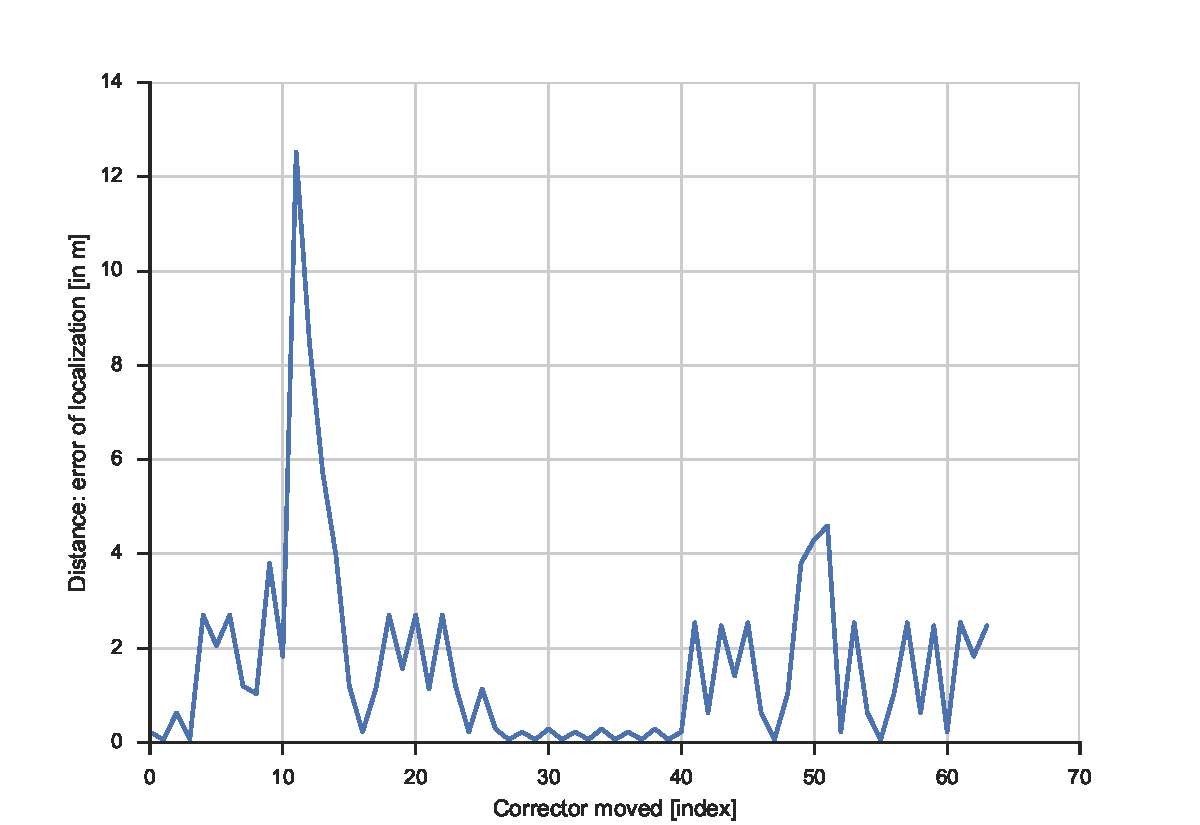
\includegraphics[width=\linewidth]{img/loc_all_y}
            \caption{Vertical}
        \end{subfigure}

    \caption{\label{fig:loc_all_corr} Localization error for all correctors}
\end{figure}

\subsection{10 Hertz harmonic perturbation}
This e

\renewcommand\cftappendixname{\appendixname~}
%%
%  Bibliography
%%
\bibliographystyle{IEEEtran}
\bibliography{tex/biblio}

\appendix
\renewcommand{\appendixname}{}
\appendixpage
% !TeX encoding = UTF-8
% !TeX spellcheck = en_US
% !TeX root = ../MasterThesis_OlivierChurlaud_2016.tex

\chapter{Mathematical appendices}
\section{Brightness and brilliance}
\label{apx:brightness_brilliance}
In the following section, the $\theta$ subscript is either $x$ or $y$.

The quality of the beam is described by the \emph{brightness} and the \emph{brilliance}.

Let F be the \emph{flux} of photons, normalized to a beam current of 1~A
\begin{equation}
F = \frac{\text{photons}}{\text{s 0.1\% BW A}},
\end{equation}

The brightness describes the angular divergence of the beam (given by $\sigma_\theta'=\sqrt{\frac{\varepsilon_\theta}{\beta_\theta}}$). It is defined as:
\begin{equation}
S = \frac{F}{2 \pi \sigma'_x \sigma'_y} = \frac{F \sqrt{\beta_x \beta_y}}{2 \pi \sqrt{\varepsilon_x \varepsilon_y}} = \frac{\text{photons}}{\text{s 0.1\% BW mrad$^2$ A}}
\end{equation}
while the brilliance includes also the transverse dimensions ($\sigma_\theta=\sqrt{\varepsilon_\theta \beta_\theta}$):
\begin{equation}
B = \frac{F}{4 \pi^2 \sigma_x \sigma_y \sigma'_x \sigma'_y} = \frac{F}{4 \pi^2 \varepsilon_x \varepsilon_y} = \frac{\text{photons}}{\text{s 0.1\% mm$^2$ BW mrad$^2$ A}}
\end{equation}

These definitions vary in literature. These are taken from the book of K.~Wille~\cite{book:wille}, and apply to Gaussian-shaped electron beams. The invariant idea is that both values are determinated by the beam emittance $\sigma$: the design of the accelerators and the correction are aimed at obtaining the smallest emittance $\varepsilon_\theta$ as possible.

\section{Principal components analysis -- Karhunen-Loève transform (KLT)}
\label{apx:KLT}

Let $\mat{X}$ be a signal with n dimensions.

\begin{equation}
\mat{X} = \left[
\begin{array}{@{}c|c|c|c@{}}
&&&\\ \vec{X}_1 & \vec{X}_2 & \dots & \vec{X}_n \\ &&&
\end{array}
\right]
\end{equation}

The covariance matrix is extracted
\begin{equation}
\mat{A} = \text{covar}(X)
\end{equation}
and diagonalized so that the eigenvalues are sorted in a decreasing order (the first one being the most significant). The covariance being symmetric, it is always diagonalizable in $\mathbb{R}$.
\begin{equation}
\mat{D} = \mat{P}^{t} \mat{A} \, \mat{P}
\end{equation}

The principal components are
\begin{equation}
\hat{\mat{X}} = \mat{P}^{t} \mat{X}
\end{equation}
and in the first column of the matrix is the most significant one.

\chapter{mBox++}
\label{apx:mbox}
The program that was handling the correction computation (see \cref{sec:correction_sa_technical}) was written in \textsc{Matlab}. It had 2 main drawbacks:
\begin{itemize}
    \item it was not very fast. \textsc{Matlab} being an interpreted language, it produces slower programs than a compiled one such as C or C++.
    \item it was difficult to extend. The code was written in a very functional way, making it hard to had debugging outputs, timers or other modules. If this can be done in \textsc{Matlab}, it is however not the easiest programming language to do it.
\end{itemize}

The program was thus rethought and rewritten from scratch. It can be found at
\begin{center}
    \url{https://github.com/ochurlaud/MSc_FOFB-mBox},
\end{center} 
licensed with the GNU General Public License v2.

\section{Specifications}

\subsection{Constrains}
\begin{itemize}
    \item mBox++ must work without any change in the current architecture and environment
    \item mBox++ must be easily maintainable and improved: modularized, encapsulated and namespaced code (e.g. object oriented) is needed (global scope must not be used to much to be able to trace variable evolutions)
\end{itemize}

\subsection{Performance}
\begin{itemize}
    \item mBox++ must be able to provide the same results as the \textsc{Matlab} version, and better in extended modes
    \item mBox++ must be at least as fast as the \textsc{Matlab} version
    \item mBox++ must be robust (e.g. graceful exit when requested, no crash on error/exception)
\end{itemize}

\subsection{Features}
\begin{itemize}
    \item mBox++ must have a \textit{read only} mode where it computes the correction but has no influence on the environment
    \item mBox++ must provide an experimental mode (where the correction is handled by external scripts)
    \item mBox++ must be able to communicate with external programs and to share its data.
    \item Tools to debug/profile must be provided
\end{itemize}

\section{Technology used}

\subsection{Language and paradigm used}
\begin{description}
    \item[Technology:] C++, Standard Template Library (STL)
    \item[Rationale:] Compiled language, thus faster than \textsc{Matlab} or Python. It is higher level than C and thus more manageable. It supports and eases object oriented programming, which allows encapsulation and to organize the code in business objects (e.g. one class is called \textit{Logger} and deals with the logs and debug strings, another acquire the data qnd is called \textit{ADC}..). Every needed types exist in the STL (vectors, strings, etc.) and it is a widely used library very well documented and experienced. The C++\,11 version is used as it provides several improvements compared to previous ones and is now available on most platforms.
    \item[Resources:] \url{http://www.cplusplus.com} --- \url{http://en.cppreference.com}
\end{description}

\subsection{Algebra computation}
\begin{description}
    \item[Technology:] Armadillo
    \item[Rationale:] Open source C++ library which API is close to \textsc{Matlab}'s and supports multi-thread calculation. It is a long tested technology (currently version 7.x) with a large and active scientific community.
    \item[Resources:] \url{http://arma.sourceforge.net}
\end{description}

\subsection{External communication}
\begin{description}
   \item[Technology:] ZeroMQ\footnote{ZeroMQ is often shortened as zmq or ZMQ}
   \item[Rationale:] Multi-platform, multi-language and open source distributed messaging library. It can be used to share messages between Python, Matlab, C/C++. It is a long tested technology (currently version 4.x), with a large and active community
   \item[Resources:] \url{http://zeromq.org}
\end{description}

\subsection{Others}
\begin{itemize}
\item The program should be able to execute interpreted scripts: it uses the official Python library in C to call Python script. 
\item To ease the localization of dependency and the compilation, the CMake (\url{https://cmake.org}) build tool is used.
\end{itemize}

\section{The program: architecture and runtime scheme}

\Cref{fig:mbox_class_diag} represents the UML\footnote{Unified Modeling Language: modeling language intended to provide a standard way to visualize the design of a system (Wikipedia)} diagram of the classes that build mBox++.

\begin{sidewaysfigure}
    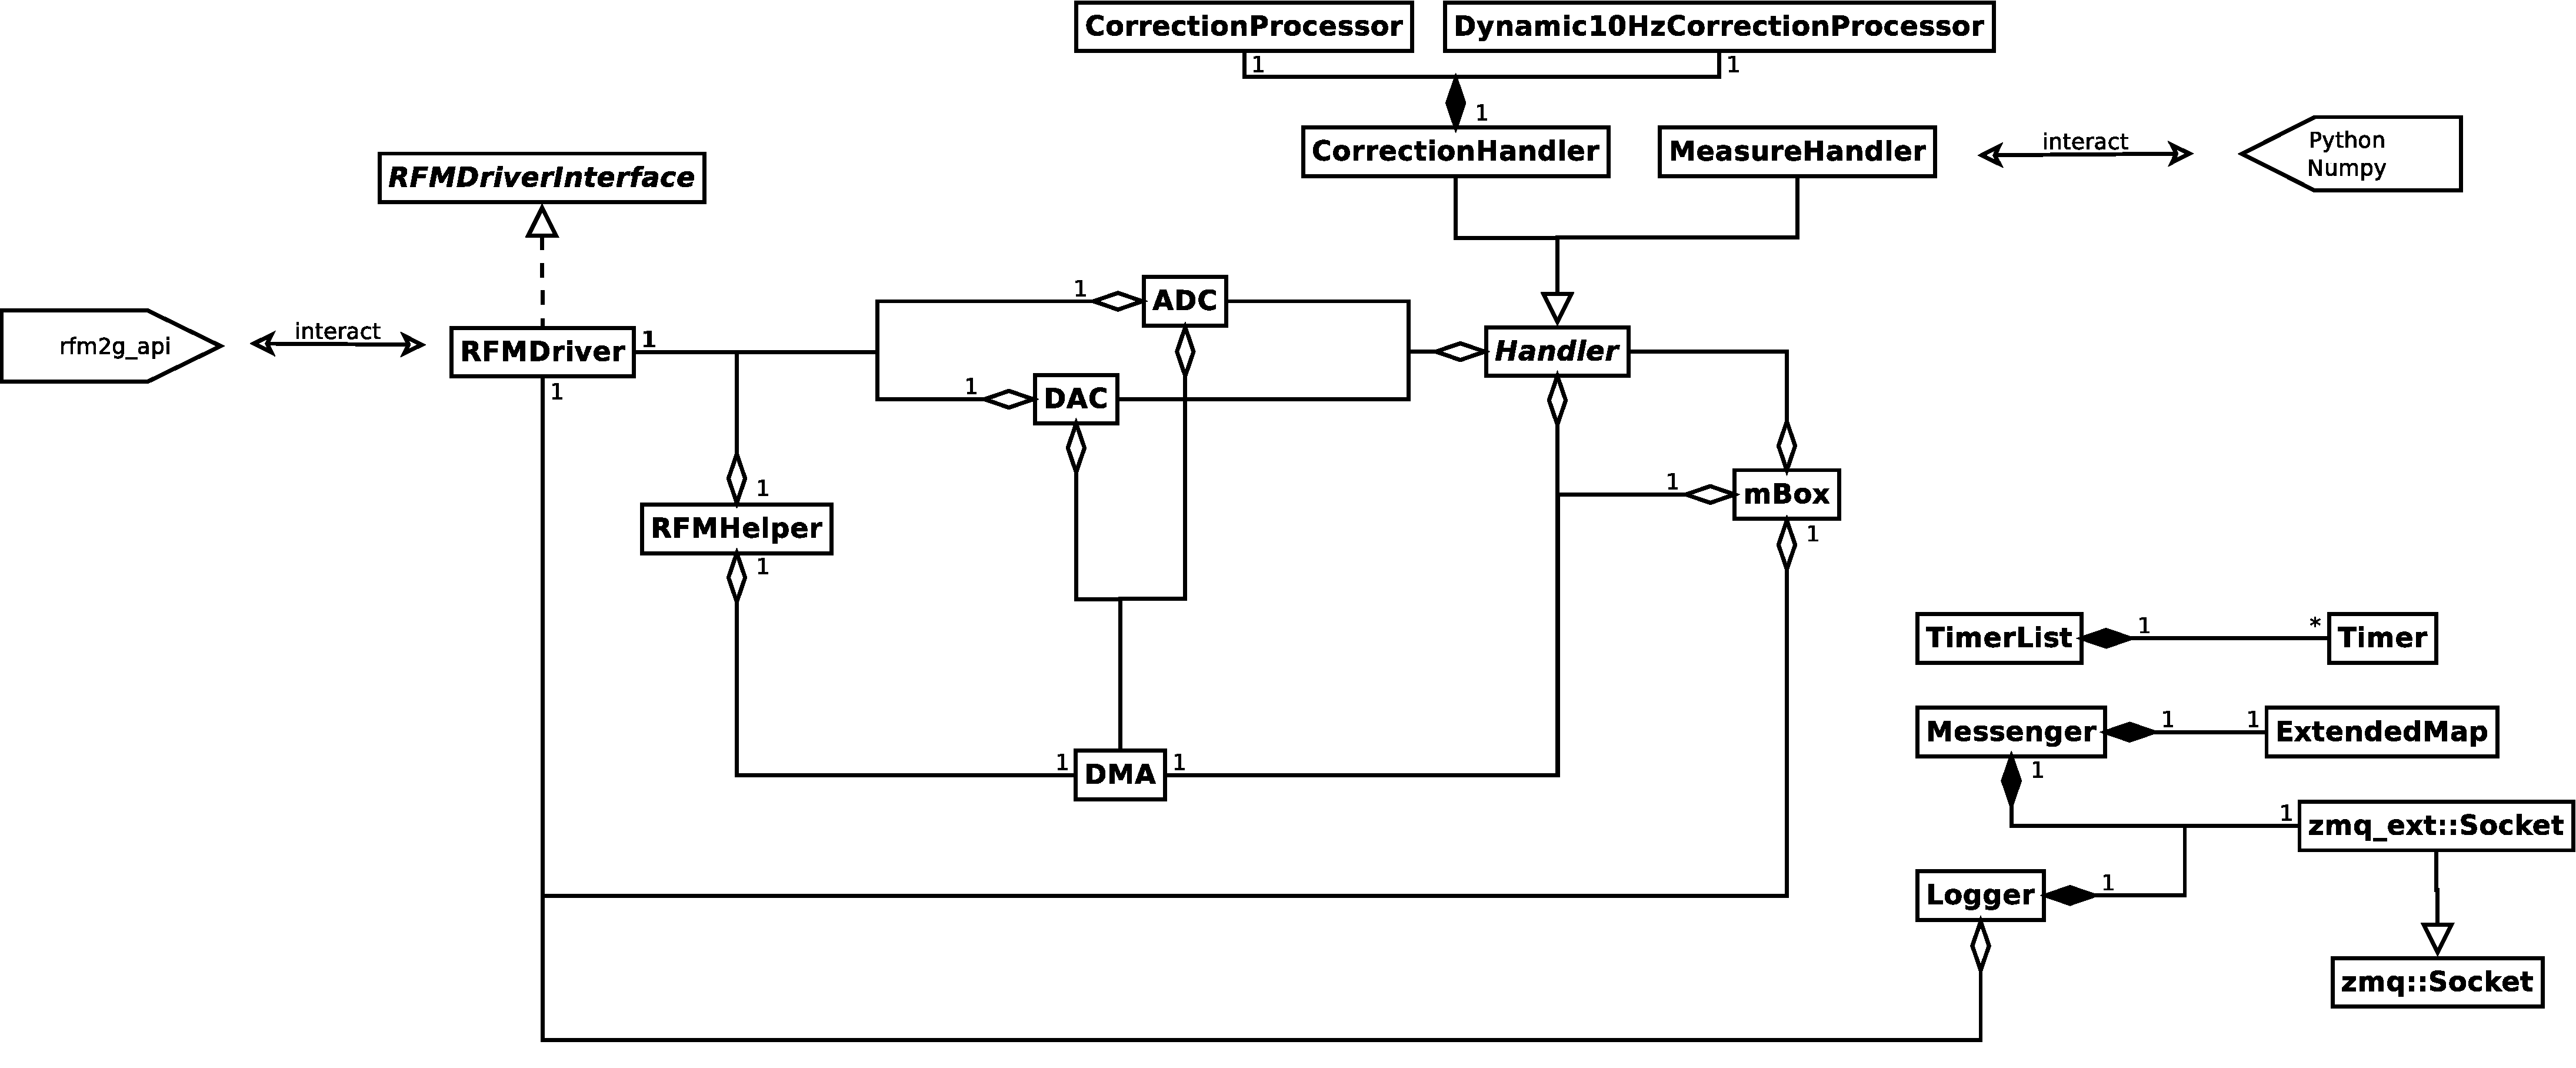
\includegraphics[width=\linewidth]{img/mBox_classDiagram}
    \caption{\label{fig:mbox_class_diag}Class diagram of the mBox++ program}
\end{sidewaysfigure}

The class \texttt{mBox} is the one from which everything begins. It creates the shared objects and deals with the state machine process. It owns a \texttt{Handler} which can be a \texttt{CorrectionHandler} if mBox++ runs in normal mode, or a \texttt{MeasureHandler} if it runs in experiment mode.

The actual mathematics (computation of the calculation) happens in the processors. If the handler is a \texttt{CorrectionHandler}, then the processor can be a \texttt{CorrectionProcessor} which does exactly what the \textsc{Matlab} code did (see \cref{sec:correction_state_of_art}) or a \texttt{Dynamic10HzCorrectionProcessor} which implements what was described in \cref{sec:dyn_corr_ex_10Hz}. Else if the handler is a \texttt{MeasureHandler}, the processor is directly the Python script provided by the user.

A handler delegates the actions to objects it owns:
\begin{enumerate}
    \item The \texttt{ADC} reads the data from the ADC reserved area in the RFM.
    \item The handler reads the data from the \texttt{ADC} object, do some conversions (mostly from a integer representation to doubles) and provides the data to its processor that calculates the correction.
    \item The correction is then converted to integers by the handler and provided to the \texttt{DAC} which writes it to the DAC reserved area in the RFM.
\end{enumerate}

To access the RFM, the C functions provided by the constructor are used. An interface \texttt{RFMDriverInterface} is implemented by the \texttt{RFMDriver} which provides a more object oriented version of the C~API.

\remark In order to be able to test the program without having access to a RFM hardware, a second \texttt{RFMDriver} (accessible by compiling with the \texttt{-DDUMMY\_DRIVER=ON} flag) implements the interface: it reads and writes in a 64~Mb binary file that represents the RFM. This can allow to create a simulation of the whole environment and to interact with the program quite easily.

Three modules are statically constructed and globally defined (in their own namespaces):
\begin{itemize}
    \item \texttt{TimerList} which is a "clever" list of \texttt{Timer}s, used to profile the parts of the code. A new or already existing timer can be started with
     \begin{c++}
         TimingModule::addTimer("name_of_timer");           
     \end{c++}
    stopped with 
    \begin{c++}
        TimingModule::timer("name_of_timer").stop();   
    \end{c++}
    and its values shown (in this case once every 1000 times) with
    \begin{c++}
        TimingModule::printAll(Timer::Unit::ms, 1000);
    \end{c++}
    The \texttt{TimimgModule} being global, it can be accessed from everywhere and thus some profiling can be done across objects and functions.

    \item \texttt{Logger} which is a class logging actions and errors. By defaults, errors only are shown to the stdout (standard output stream). Logs and errors are published on a given port (3333 by default) with ZeroMQ and can be read by subscribed services (the logs and errors can thus be output, saved in a file, published on a website stream or whatever crazy idea the user can have). It uses the ZeroMQ Publisher mode. A debug mode is also available (see \texttt{--help} command). It publishes incoming and outgoing values that can be used by other scripts or programs for display, scripting, value-checking... The full description of the uses are given in the Doxygen\footnote{Popular documentation generator that extracts specific comments to produce PDF or HTML documentation. See \url{http://www.stack.nl/~dimitri/doxygen/index.html}} documentation
    
    \item \texttt{Messenger} which is a class for exchanging information with outside scripts and programs. It is listening on a given port (3334 by default). It is using the ZeroMQ Router mode. Every time it receives a request, it processes it and either return the value of the requested variable, or set the given variable to the received value. The difference with the \texttt{Logger} is that the logger publishes values even if no one is listening and sends it when the asked by the code, whereas the \texttt{Messenger} only answers queries. It is notably used in the harmonic correction process described in \cref{sec:dyn_corr_ex_10Hz}: a python script calculates all the phases and amplitudes and sends the outcome, which are then used by \texttt{Dynamic10HzCorrectionProcessor}.
\end{itemize}

\section{Project organization}
The project is organized as followed:
\begin{itemize}
    \item \texttt{/cmake} contains CMake modules to find other libraries and dependencies.
    \item \texttt{/doc} contains resources for the documentation and the generated documentation (which is not synchronized in the version control).
    \item \texttt{/experimentScripts} contains Python scripts that can be used as processor in experiment mode.
    \item \texttt{/python\_tools} contains Python scripts and modules that can be used with the program: the helper for the harmonic correction is there (\texttt{tenHz.py}), a module to communicate with mBox++ through a binary file in dummy mode (\texttt{cbox.py}, \texttt{dummy\_simul.py}) and various helpers to subscribe to the ZeroMQ streams, save data in a specified way...
    \item \texttt{/src} contains all the C++ code to be compiled. Its root contains the core of the project. The rest of the code is split in \texttt{/src/modules}, \texttt{/src/handlers} for a better readability.     
    \end{itemize}
Finally at the root of the project is \texttt{README.md} file giving the dependencies, how to compile, install and use mBox++. A Doxygen configuration file \texttt{doxygen.conf} let the documentation be generated by starting
\begin{verbatim}
    $ doxygen doxygen.conf
\end{verbatim}
   
\section{Use}
mBox++ cannot run if it does not receive the order from the cBox: it would else hang in a waiting state.
It can be used in normal mode
\begin{verbatim}
    $ mbox --rw
\end{verbatim}
in read only
\begin{verbatim}
    $ mbox --ro
\end{verbatim}
A full overview of the commands are given by
\begin{verbatim}
    $ mbox --help

    === mbox (2015-2016) ===
    Use:
    mbox --ro
        Read only version: just reads the RFM and calculates
        the correction, don't write it back.
    mbox --rw
        Read-write version: reads the RFM, calculates the
        correction and write it on the RFM.
    mbox --experiment <FILENAME>
        Read-write version for experiments: read the file <FILENAME>
        to know which values to create.
    
    Other arguments (to append):
    --debug
        Print the logs on the the stderr.
    --logport <PORT>
        Which port the log publisher should use.
    --queryport <PORT>
        Which port the query messenger should use.
\end{verbatim}

\chapter{Search Kick}
Search Kick was originally only able to find kicks in the orbit, in order to localize perturbation sources. It is currently closer to a Python orbit toolbox that allows translating dump data between various formats, localizing perturbations, and other small algorithms for inverting matrices or optimizing signals.

The library can be found at 
\begin{center}
        \url{https://github.com/ochurlaud/MSc_SearchKicks}
\end{center}
licensed with the GNU General Public License v2.


    

\end{document}

